\documentclass[11pt,a4paper]{article}

%\usepackage[square]{natbib}
\usepackage[utf8]{inputenc}
\usepackage[czech]{babel}

%\usepackage[T1]{fontenc}
%\usepackage{uarial}
%\renewcommand{\familydefault}{\sfdefault}
%\renewcommand{\rmdefault}{\sfdefault}
%\usepackage{sfmath}
%\usepackage{sansmath}

\usepackage{amsfonts,amsmath}
\usepackage{etoolbox}
\usepackage{graphicx}
\usepackage[unicode]{hyperref}
\usepackage{multirow}
\usepackage{titlesec}
\setcounter{secnumdepth}{3}
\usepackage{float}
\usepackage{caption}
\usepackage{subcaption}
\usepackage{setspace}
\usepackage{geometry}
\usepackage{calc}
\usepackage{booktabs}


\geometry{verbose,
          tmargin=4cm,
          bmargin=3cm,
          lmargin=2.5cm,
          rmargin=2.5cm,
          footskip=24pt}
% \newlength\mytopmargin
% \newsavebox{\headbox}\savebox{\headbox}{
%   \begin{flushleft}                           
%   
\includegraphics[width=2cm]{logo_TACR_zakl.pdf} 
%   \end{flushleft}}
% \setlength{\mytopmargin}{\totalheightof{\usebox{\headbox}}+2cm}
% \geometry{verbose,
%           tmargin=\mytopmargin,
%           headheight=1.1\mytopmargin}
% \usepackage{fancyhdr}
% \fancyhf{}
% \fancyhead[C]{\usebox\headbox}
% \renewcommand{\headrulewidth}{0pt}
\usepackage{fancyhdr}
\pagestyle{fancy}
\renewcommand{\headrulewidth}{0pt}
\fancyhead[L]{\begin{picture}(0,0) 
\put(0,0){
\includegraphics[width=2cm]{logo_TACR_zakl.pdf}} 
\end{picture}}% empty left


% \usepackage{fancyhdr}
% %\pagestyle{fancy}
% \fancyhead{
% %     \begin{picture}(0,0)
% %         \put(-20,-10)
% %     \end{picture}
%     {
\includegraphics[width=2cm]{logo_TACR_zakl.pdf}}
%     \vbox{
%       Technologická agentura\\
%       České republiky
%     }
%     }
% \rhead{}    
% \cfoot{}
% \rfoot{\thepage}
% \renewcommand{\headrulewidth}{0pt}

\newcommand{\obraz}[1]{(viz obr. \ref{#1})}
\newcommand{\tabul}[1]{(viz tab. \ref{#1})}
\newcommand{\pozn}[1]{(viz odst. \ref{#1})}


\usepackage{tikz}

% macro for units.
\def\UNIT#1#2{\ifstrempty{#2}{}{%
\ifstrequal{#2}{1}{\mathrm{#1}}{\mathrm{#1}^{#2}}%
}}
\def\units#1#2#3{\ifstrempty{#1#2#3}{$[-]$}{$[ \UNIT{kg}{#1}\UNIT{m}{#2}\UNIT{s}{#3} ]$}} %with brackets
\def\unitss#1#2#3{\ifstrempty{#1#2#3}{$-$}{$ \UNIT{kg}{#1}\UNIT{m}{#2}\UNIT{s}{#3} $}}    %without brackets

%macro for hyperlinks (dummy)
\def\hyperA#1#2{#2}
  


% ***************************************** SYMBOLS
\def\abs#1{\lvert#1\rvert}
\def\argdot{{\hspace{0.18em}\cdot\hspace{0.18em}}}
\def\bb{\vc b}
\def\d{\mathrm{d}}
\def\D{{\tn D}}
\def\div{\operatorname{div}}
\def\grad{\nabla}
\def\jmp#1{[#1]}
\def\n{\vc n}
\def\nn{\vc n}
\def\prtl{\partial}
\def\R{\mathbb R}
\def\Real{\mathbb R}
\def\sc#1#2{\left(#1,#2\right)}
\def\th{\vartheta}
\def\tn#1{{\mathbb{#1}}}    % tensor
\def\vc#1{\mathbf{\boldsymbol{#1}}}     % vector
\def \E{{\mathsf E}}
\def\avg#1{\langle#1\rangle}
\def\var#1{\llangle#1\rrangle}
\def\Var{\mathop{\rm Var}}
\def\Cov{\mathop{\rm Cov}}
%\def\log{\mathop{\rm log}}
\def\abs#1{|#1|}

\def\vl{{\vc\lambda}}
\def\estvl{{\vc{\hat\lambda}}}
\def\estrho{\hat\rho}
\def\vmu{\vc\mu}
\def\estvmu{{\vc{\hat\mu}}}
\def\vphi{\vc\phi}

\newcommand{\jb}[1]{{\color{violet} JB: #1}}
%***************************************************************************





\begin{document}
\begin{onehalfspacing} 

%\ULCornerWallPaper{1}{\includegraphics{TACR_logo.png}}
%\LLCornerWallPaper{1}{bar}
%\lipsum[1-3]

\begin{titlepage}
    
\includegraphics[width=2cm]{logo_TACR_zakl.pdf}

    \vspace{6cm}
    {\centering	
      {\scshape\bf\huge Model transportu v okolí úložných vrtů\par}
      \vspace{3cm}
      
      {\LARGE Petr Rálek}
      
      \vspace{1cm}
      {\LARGE 2020}
      
    }
    \vfill
% Bottom of the page
\end{titlepage}

%\setcounter{page}{4}


\section{Popis modelu}

Model transportu popisuje šíření kontaminantu oblastí úložiště se zahrnutím EDZ a stochasticky generované puklinové sítě. Předpokladem je, že EDZ kolem úložných vrtů zesiluje průtoky podzemní vody podél těchto vrtů.

V hierarchii kontejner/bentonit/edz/úložiště/masiv/biosféra se model nachází mezi úrovněmi rozhraní bentonit/edz a vnější hranicí úložiště (či spíše ještě několika desítek metru dále). Pracuje s výsledky modelů dalších úrovní \obraz{schema_modelu}: a) jako zdrojový člen kontaminace slouží výsledky samostatného modelu blízkého pole (převzato), b) hydraulické podmínky na hranici oblasti úložiště jsou převzaty z regionálního hydrogeologického modelu \cite{riha_hradek}. 

Hlavním výstupem modelu by měla být časová řada koncentrace kontaminantu na vnější hranici úložiště,
na které jsou založeny indikátory bezpečnosti EDZ navžené v rámci projektu.

%(kterou lze využít jako zdrojový člen regionálního modelu transportu.) \jb{To lze, ale cílem v rámci projektu je použití pro výpočet odvozených indikátorů bezpečnosti.}

\begin{figure}[H]
\centering
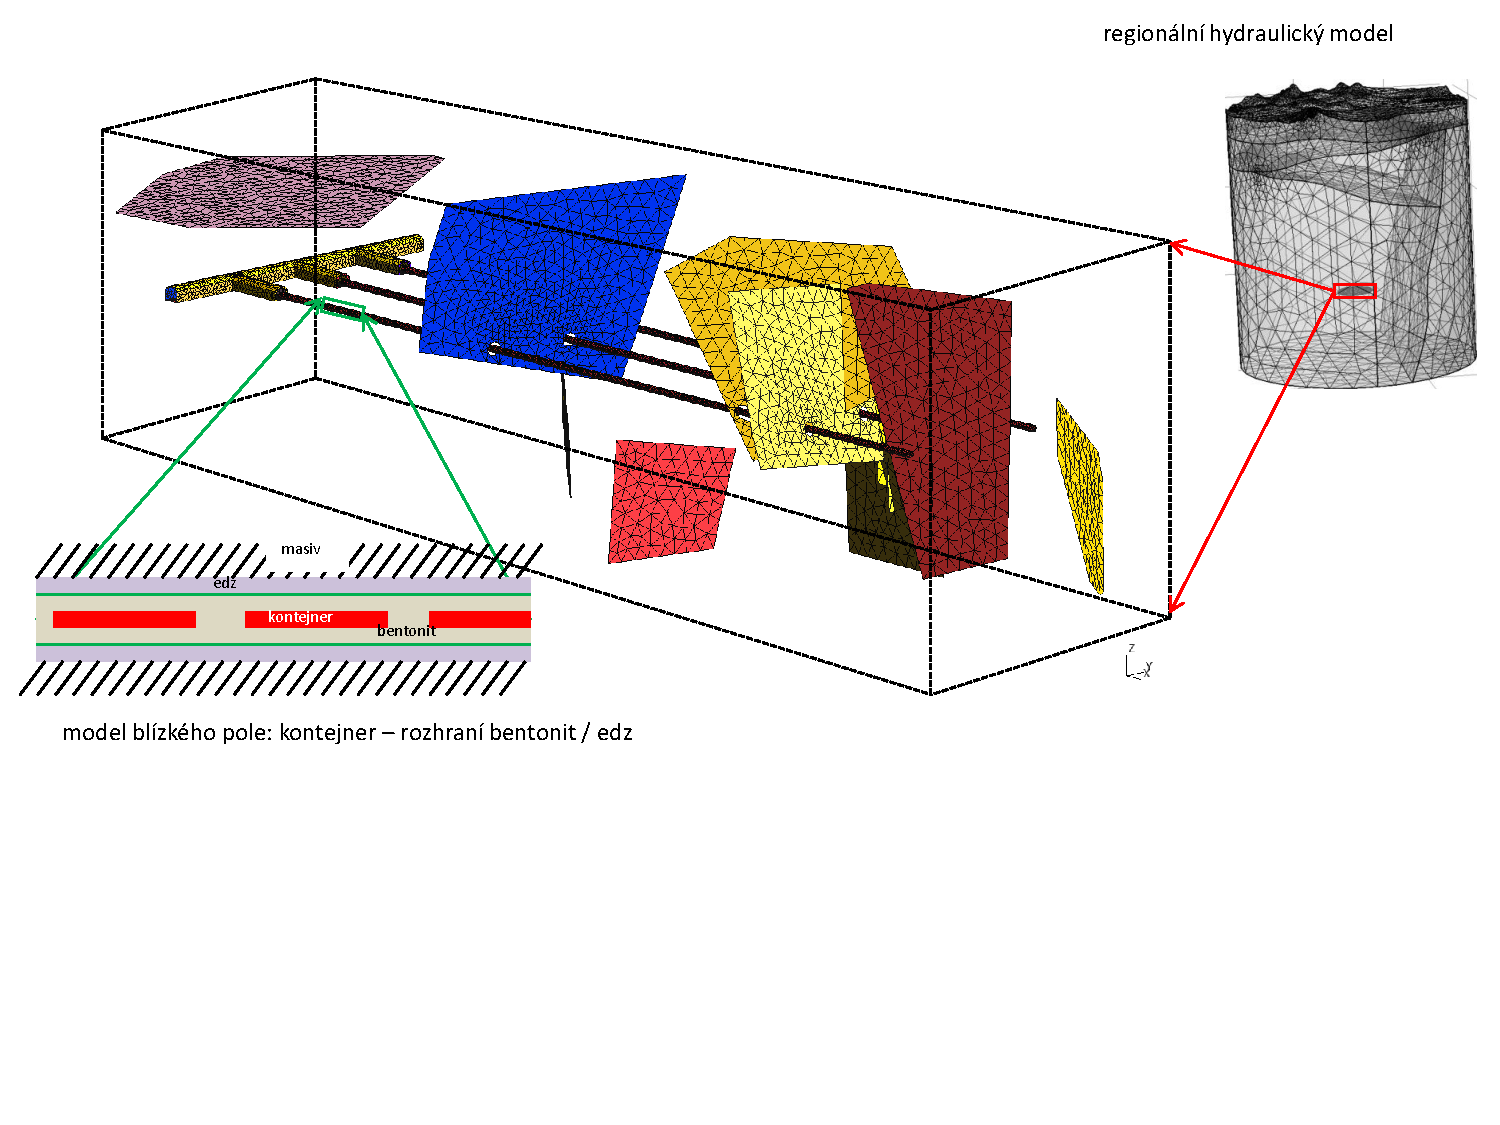
\includegraphics[width=16cm]{graphics/obr_ralek/schema_modelu01.pdf}
\vspace{-4.5cm}
\caption{Geometrie (části) úložiště s převzatými okrajovými podmínkami z~dalších modelů.}
\label{schema_modelu}
\end{figure}

\newpage

\subsection{Geometrie modelu}

\begin{figure}[ht]
\centering
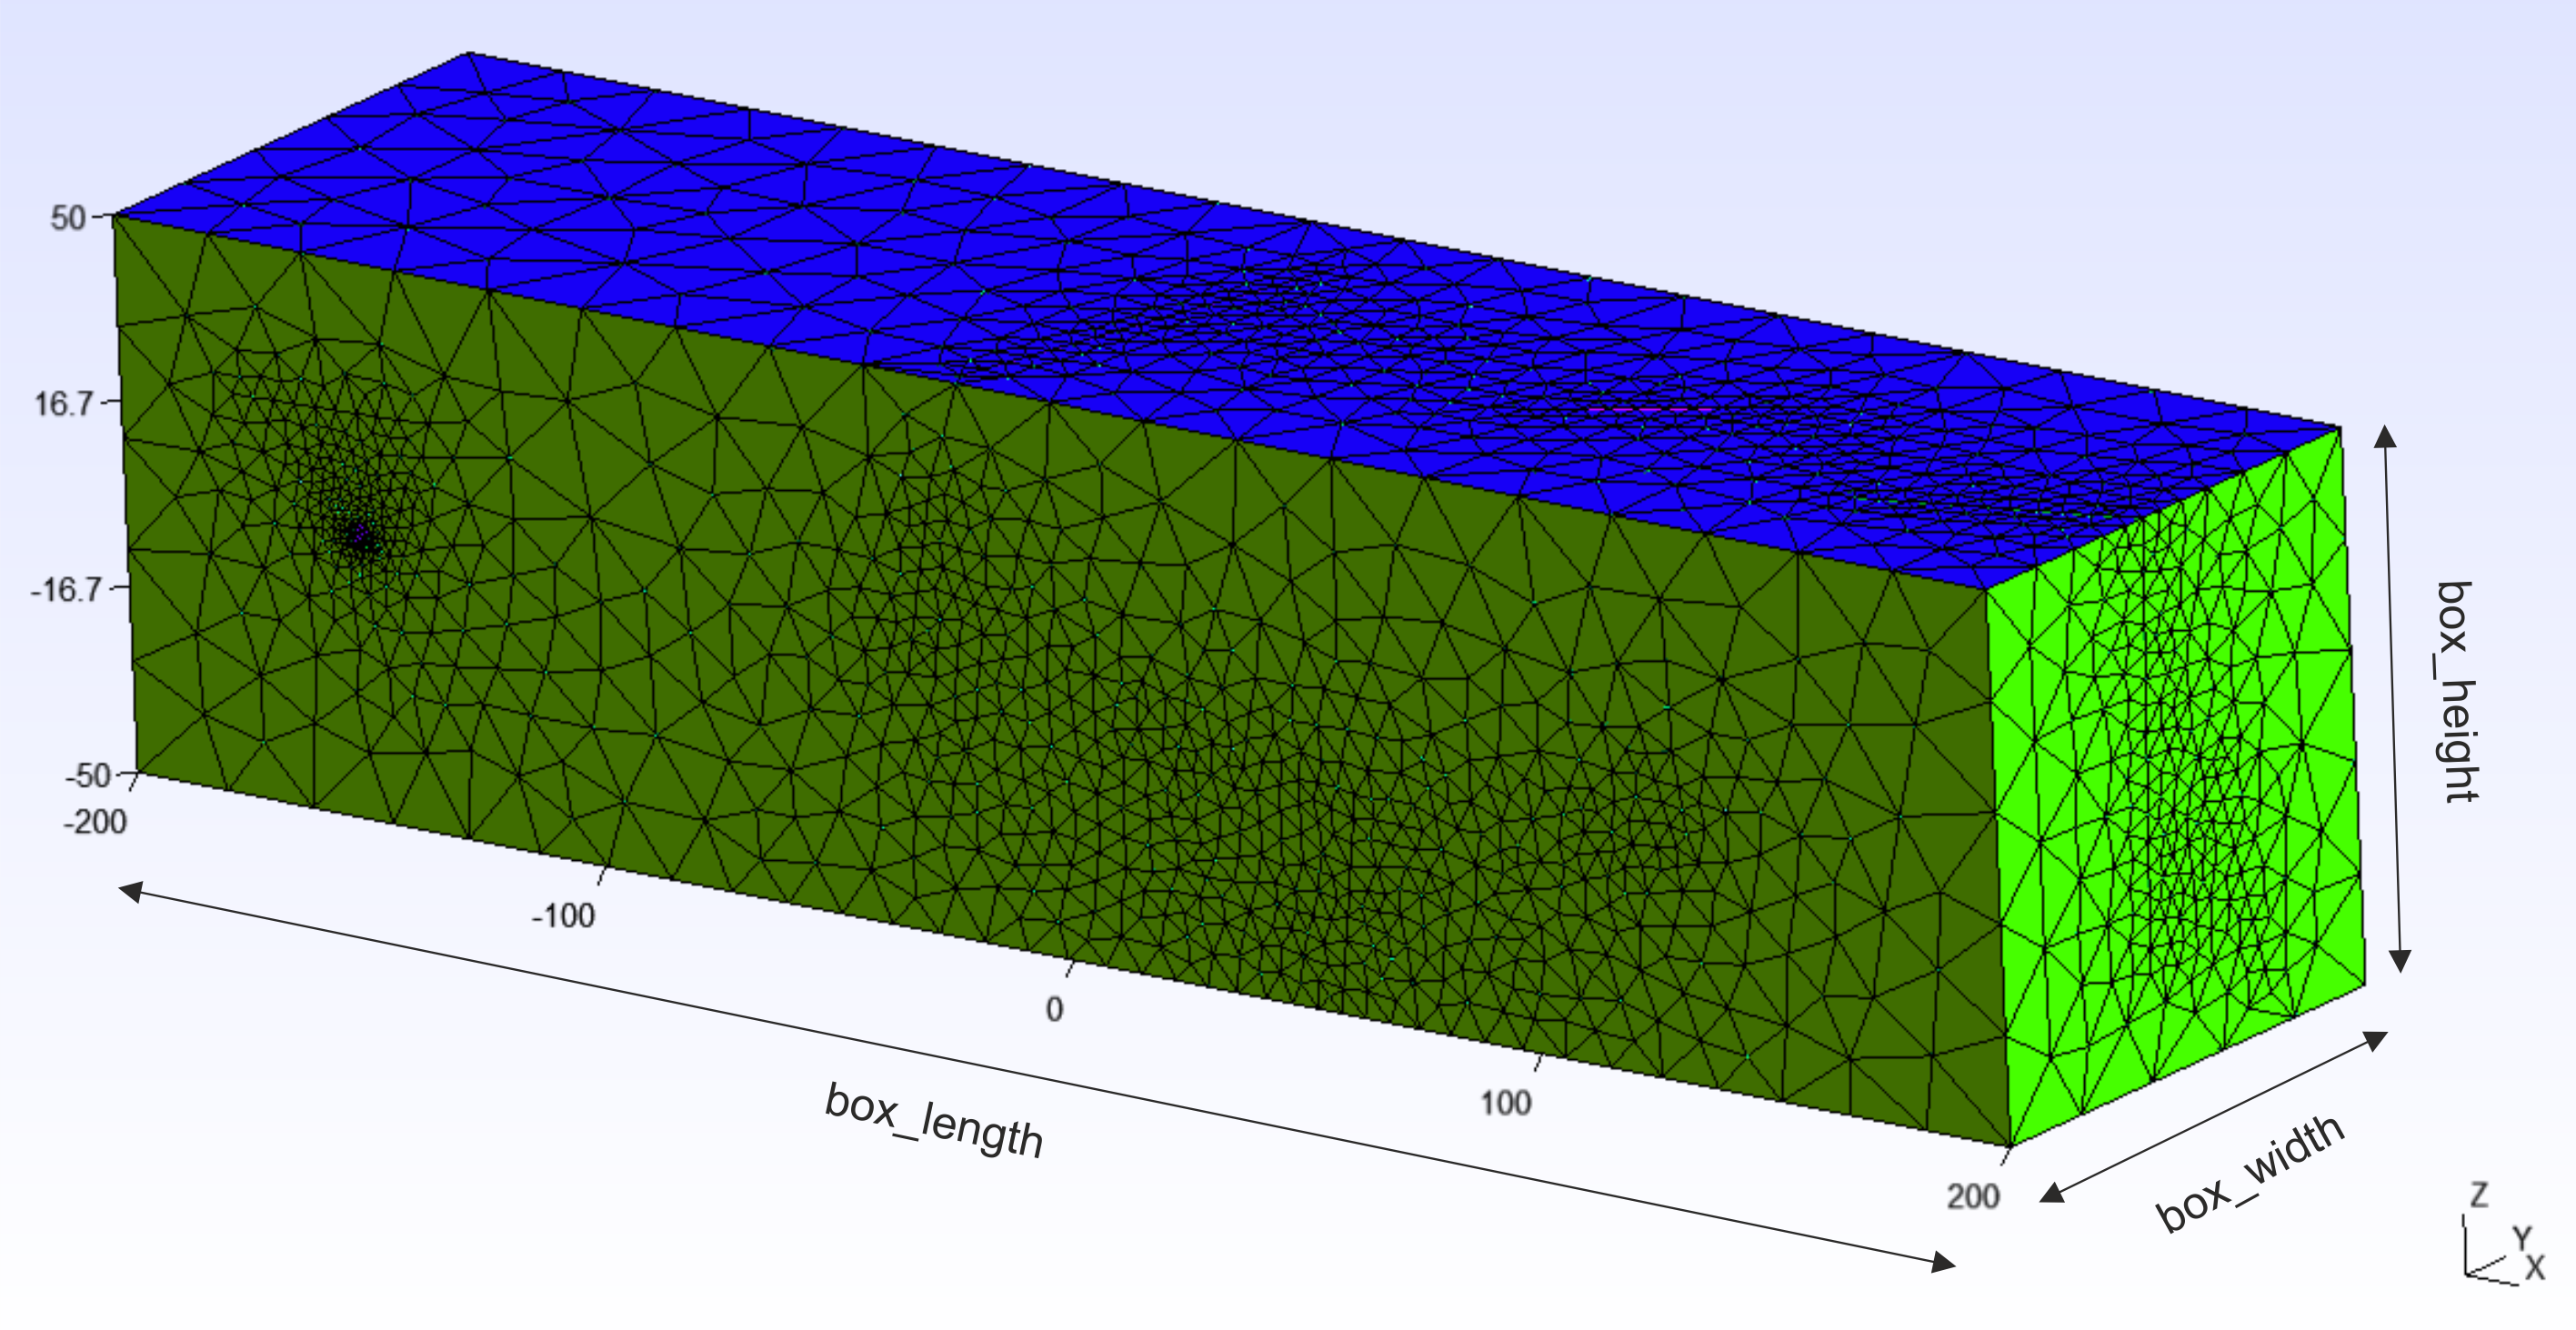
\includegraphics[height=4.2cm]{graphics/obr_ralek/box_okotovany.png}
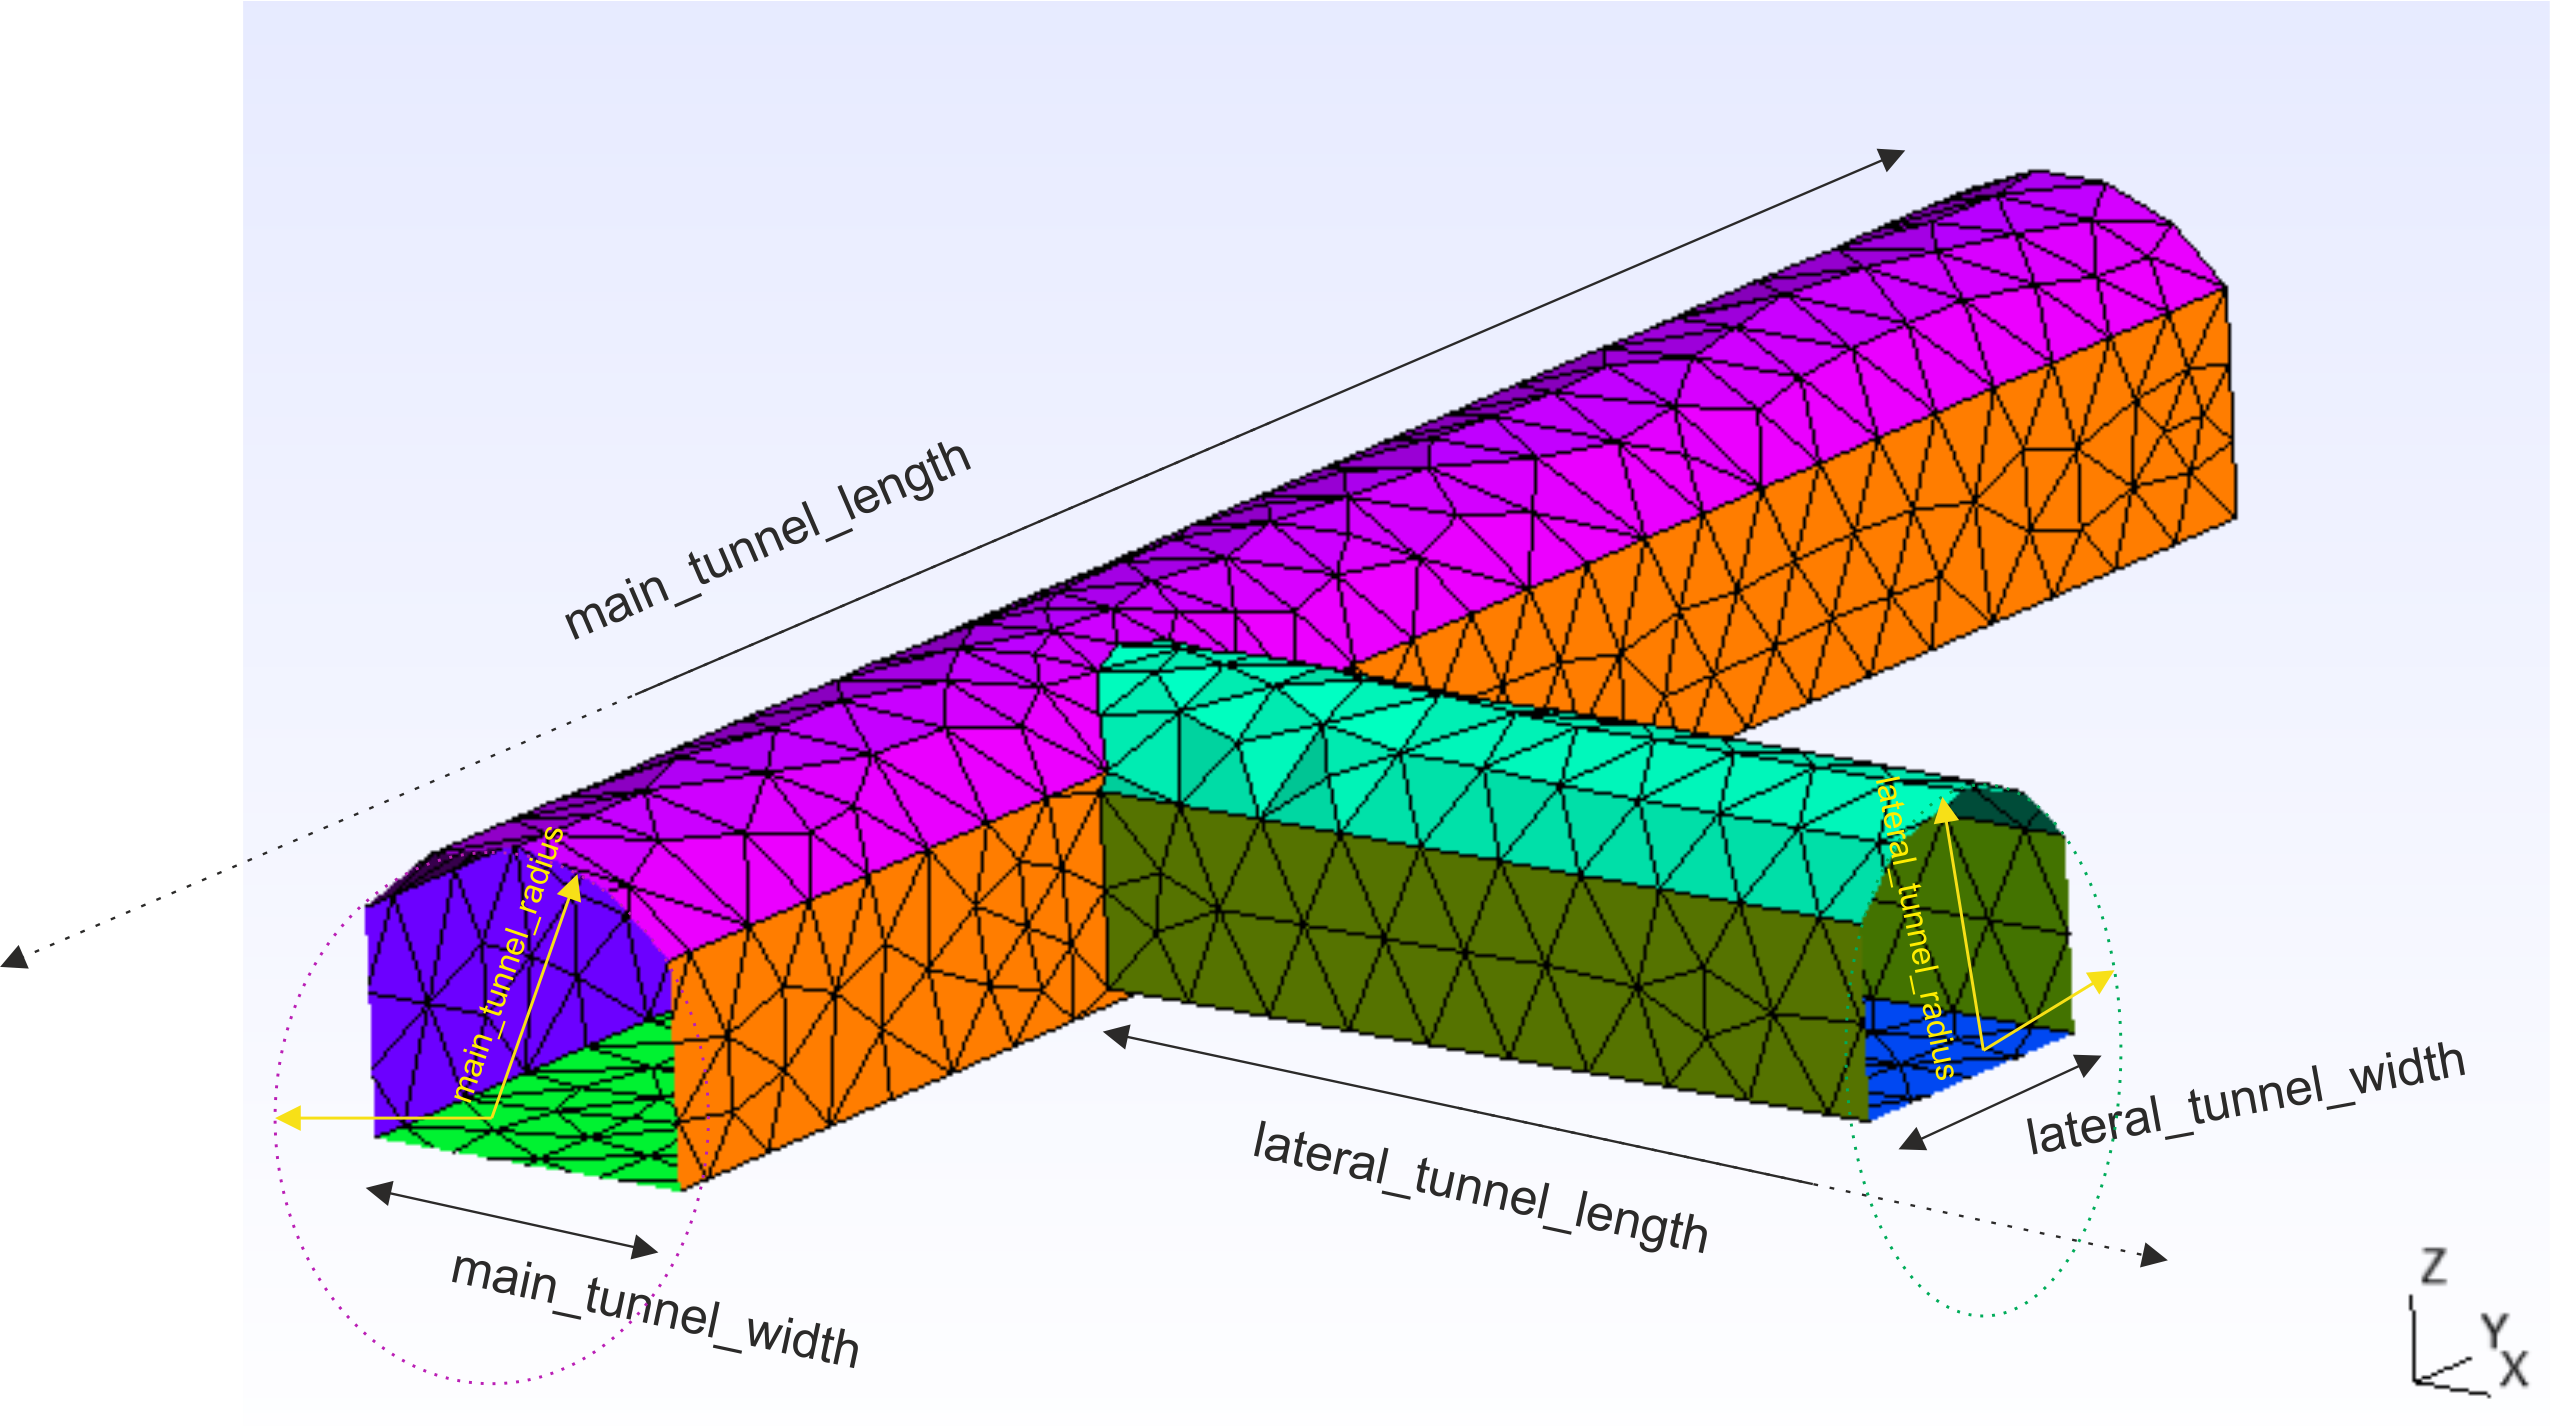
\includegraphics[height=4.2cm]{graphics/obr_ralek/main_tunnel_rez_okotovany.png}
\\
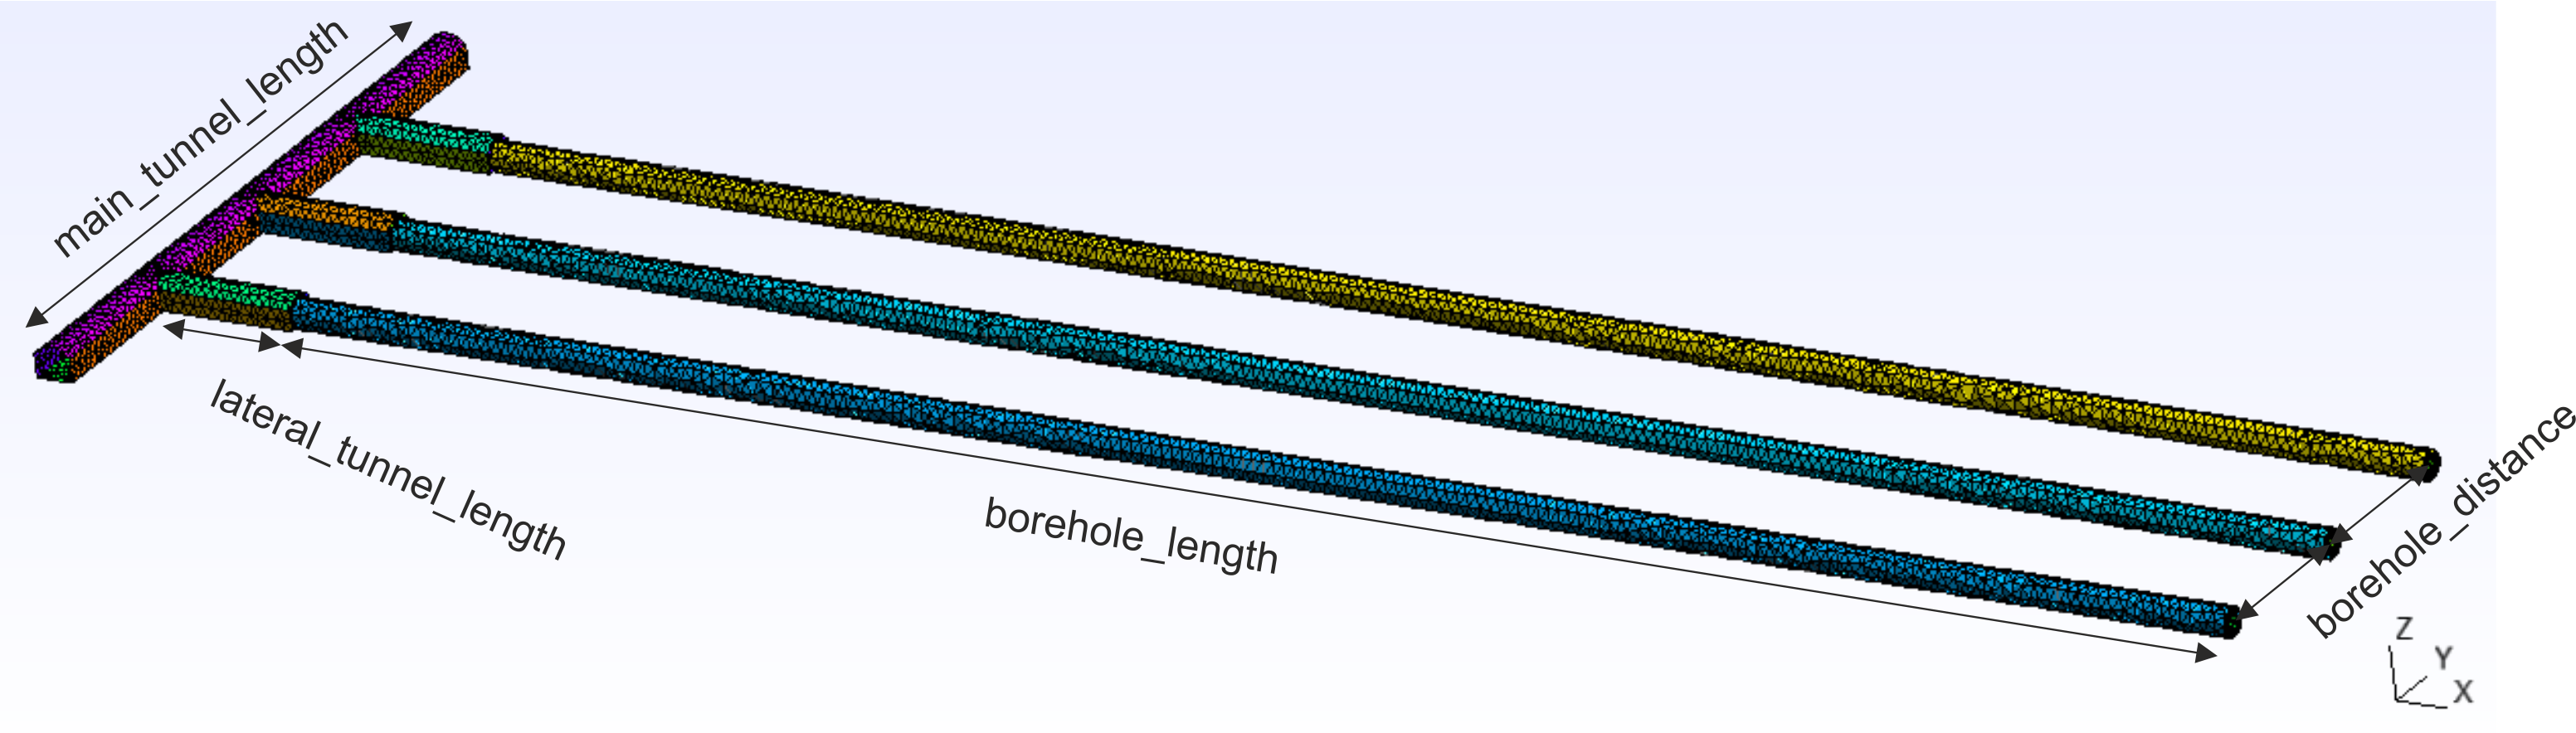
\includegraphics[height=3.1cm]{graphics/obr_ralek/boreholes_okotovane.png}
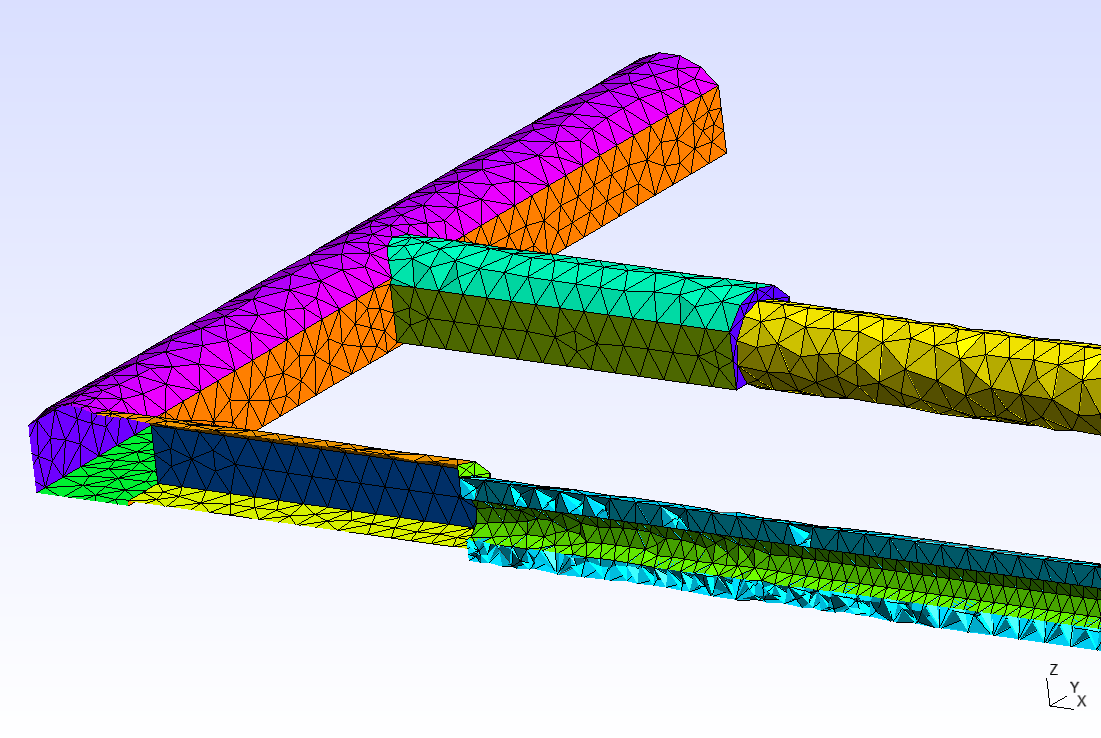
\includegraphics[height=3.1cm]{graphics/obr_ralek/rez_podel.PNG}
\caption{Jednotlivé části geometrie modelu (bez puklin). Vlevo nahoře: celý modelovaný blok masivu. Vpravo nahoře: hlavní rozrážka s~bočními tunely (výřez). Vlevo dole: hlavní rozrážka s~bočními tunely a~horizontálními úložnými vrty s~vrstvou edz. Vpravo dole: vertikální podélný řez prostředním vrtem s~viditelnou vrstvou edz.}
\label{geom_okotovana}
\end{figure}
\vspace{-0.5cm}

\begin{table}[ht]
\begin{center}
    \caption{Použité rozměry geometrie.}
    \begin{tabular}{ | l | c |}
    \hline
    \small parametr & \small rozměr [m] \\ \hline
    \small box\_length & \small 400 \\ \hline
    \small box\_width & \small 100 \\ \hline
    \small box\_height & \small 100 \\ \hline
    \small edz & \small 2 \\ \hline
    \end{tabular}
    \begin{tabular}{ | l | c |}
    \hline
    \small parametr & \small rozměr [m] \\ \hline
    \small borehole\_length & \small 300 \\ \hline
    \small borehole\_distance & \small 25 \\ \hline
    \small borehole\_radius & \small 1.1 \\ \hline
    \small main\_tunnel\_length & \small 100 \\ \hline
    \end{tabular}
    \begin{tabular}{ | l | c |}
    \hline
    \small parametr &  \small rozměr [m] \\ \hline
    \small main\_tunnel\_width & \small 5.5 \\ \hline
    \small main\_tunnel\_radius & \small 3.5 \\ \hline
    \small lateral\_tunnel\_length & \small 23 \\ \hline
    \small lateral\_tunnel\_width & \small 5 \\ \hline
    \small lateral\_tunnel\_radius & \small 3 \\ \hline
    \end{tabular}
    \label{tab_parametry_geom}
\end{center}
\end{table}
\vspace{-0.3cm}

V současném stavu zahrnuje geometrie modelu výřez masivu úložiště s jednou hlavní a~třemi bočními rozrážkami, na které navazují horizontální ukládacími vrty. Vlastní objemy rozrážek a~vrtů nejsou součástí výpočetní sítě (tvoří prázdný prostor v~masivu). Rozměry modelované oblasti a jejích částí \obraz{geom_okotovana} jsou volitelnými parametry. Použité rozměry rozrážek odpovídají předpokládaným skutečným rozměrům. Tloušťka EDZ (2~m) je v~současné verzi nadhodnocena z~důvodu snazší diskretizace\footnote{Současná verze geometrie modelu se potýká s několika nedostatky. Východiska a plán dalších prací jsou diskutovány samostatně v odstavci \ref{detskenemoci} na konci této kapitoly.}.

K tvorbě sítě je využita knihovna BGEM (vlastní vývoj) zpřístupňující procedury programového rozhraní balíku GMSH \cite{gmsh}. 

Celý proces zatím nebyl odladěn tak, aby vysíťování oblasti bylo dostatečně robustní. Úspěšnost síťování (s~parametry v tabulce \ref{kroky_site}) geometrie pro různé varianty stochasticky generované puklinové sítě o~několika desítkách puklin se pohybovala pouze okolo 10-20~\% \pozn{detskenemoci}. K~výpočtům byly použity geometrie s~cca 10 puklinami o~velikosti mezi 400 - 500 tis. elementy. 

\begin{table}[ht]
\begin{center}
    \caption{Parametry pro řízení kroků sítě.}
    \begin{tabular}{ | l | c |}
    \hline
    \small parametr & \small maximální velikost [m] \\ \hline
    \small fracture\_mesh\_step & \small 5 \\ \hline
    \small boundary\_mesh\_step & \small 20 \\ \hline
    \small borehole\_mesh\_step & \small 0.8 \\ \hline
    \small main\_tunnel\_mesh\_step & \small 1.5 \\ \hline
    \end{tabular}
    \label{kroky_site}
\end{center}
\end{table}
\vspace{-0.3cm}

\begin{figure}[H]
\centering
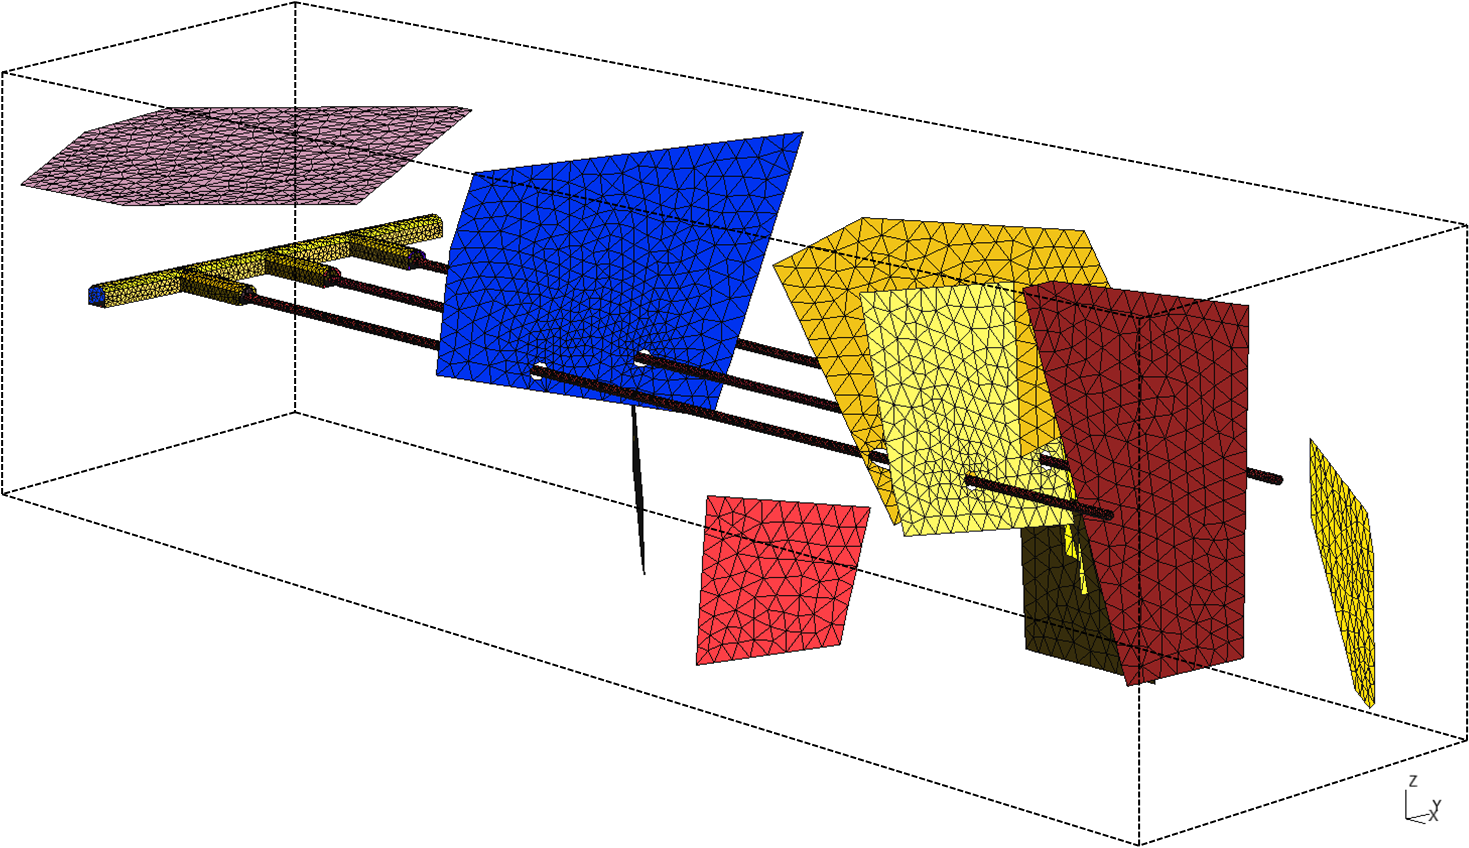
\includegraphics[width=16cm]{graphics/obr_ralek/geom02.png}
\caption{Geometrie modelu se stochasticky generovanou puklinovou sítí (bez zobrazené edz).}
\label{geom02}
\end{figure}

% \newpage
% \subsection{Konceptuální model}
% \begin{itemize}
%     \color{red}
%     \item Advektivně-difúzní transport, zatím použitá jen advekce
%     \item odkazy na konkrétní knihovny flow123d?
% \end{itemize}
% \jb{Zde by bylo dobré popsat konceptuální model, t.j. model proudění, jaké je kde volená/vlitelná vodivost, jaké OKP. A dále data modelu transportu, zmínit řešení pomocí DG metody.}

\subsubsection{Okrajové podmínky}
     \begin{enumerate}
        \item hydraulické OP (\cite{flow_pdf_manual}, str. 28):
            \begin{itemize}
                \item nulový tok přes vnější hranice vrtů,
                \item nulový tok přes hranice tunelu a rozrážek (počítá se se zalitím stěn rozrážek pryskyřicí a následným vybetonováním rozrážek),
                \item tlaková výška na vnější hranici modelované oblasti převzatá z regionálního modelu
            \end{itemize}
        \item transportní OP (\cite{flow_pdf_manual}, str. 31):
            \begin{itemize}
                \item zadaný tok koncentrace $\sigma_c~[kg.m^{-2}.s^{-1}]$ přes (části) vnější hranice vrtů,
                \item nulová koncentrace a nulový tok koncentrace přes hranice tunelu a rozrážek,
            \end{itemize}
     \end{enumerate}
     
Transportní úloha je řešena nespojitou Galerkinovou metodou (viz \cite{flow_pdf_manual}, str. 46), implementovanou v balíku Flow123d \cite{flow123d}.



\newpage
\section{Testovací úlohy}

Testovací úlohy měly mj. prokázat přenositelnost vnějších (hydraulických) a vnitřních (transportních) okrajových podmínek (OP) z~externích modelů:
\begin{itemize}
\item Hydraulické OP na hranici oblasti byly převzaty z modelu lokality Hrádek \cite{riha_hradek}. Na obrázku \ref{hradek_piezo_head_orez} je znázorněno rozložení piezometrické výšky v~předpokládané úrovni úložiště a~vyznačena poloha geometrie (s~rozměry box\_length a~box\_width).
\item Jako zdrojový člen kontaminace je zadán tok koncentrace kontaminantu v čase na povrchu (části\footnote{Toto je jeden z nedostatků současné verze modelu, Flow123d zatím neumí pracovat s časově proměnnou OP na části geometrie zadané souřadnicemi (viz odstavec \ref{detskenemoci}).}) úložného vrtu. 

Byly spočteny úlohy se třemi variantami OP:
    \begin{enumerate}
        \item Konstantní zdroj $\sigma_c=10^{-6}~kg.m^{-2}.s^{-1}$ na části prostředního vrtu o délce 10 m (odpovídající jednomu kontejneru) po celou dobu simulace.
        \item Konstantní zdroj $\sigma_c=10^{-6}~kg.m^{-2}.s^{-1}$ na všech vrtech s "vypnutím" po 10 letech (pak $\sigma_c=0$).
        \item Proměnný zdroj na všech vrtech: hodnoty toku koncentrace kontaminantu převzaty z modelu blízkého pole pro $^{129}I$ \obraz{flux_I}.
    \end{enumerate}
\end{itemize}

\begin{table}[ht]
\begin{center}
    \caption{Použité hodnoty hydraulické vodivosti a porozity.}
    \begin{tabular}{ | l | c | c |}
    \hline
    \small oblast & \small konduktivita [$\rm m^{-1}$] & \small porozita [1]\\ \hline
    \small masiv & \small $10^{-8}$ & \small 0.01\\ \hline
    \small pukliny & \small $10^{-7}$ & \small 1\\ \hline
    \small edz & \small $10^{-7}$ & \small 0.1\\ \hline
    \end{tabular}
    \label{konduktivita}
\end{center}
\end{table}
\vspace{-0.3cm}

\begin{figure}[H]
\centering
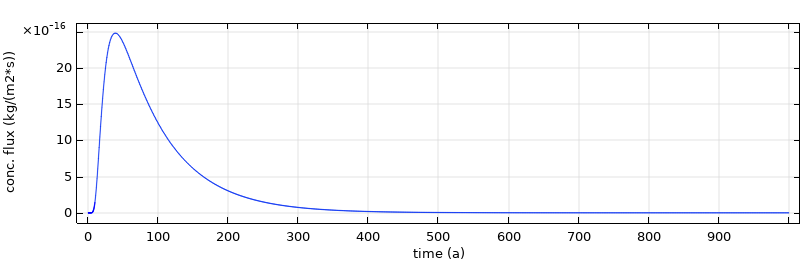
\includegraphics[width=16cm]{graphics/obr_ralek/c_flux_jod.png}
\caption{Časový průběh (prvních 500 let) hmotnostního toku izotopu $^{129}I$ z bentonitové vrstvy kolem jednoho kontejneru.}
\label{flux_I}
\end{figure}

\begin{figure}[H]
\centering
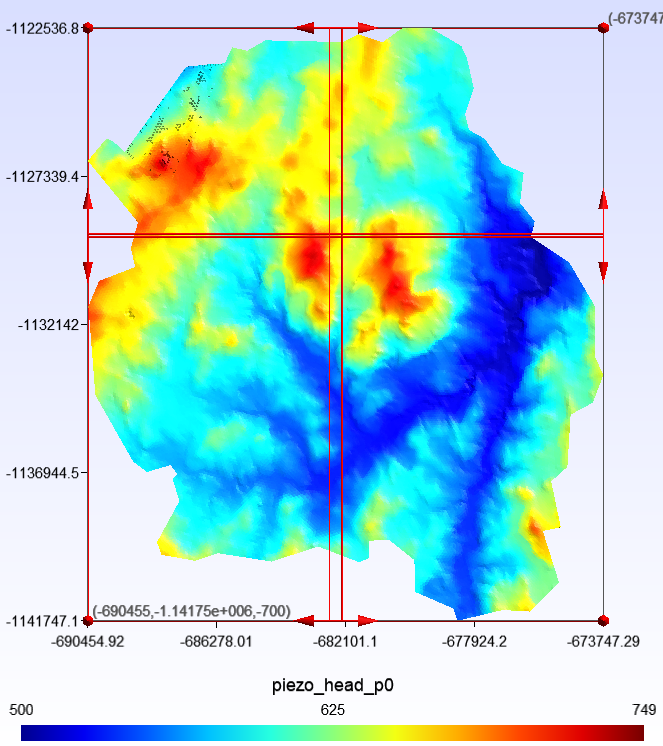
\includegraphics[width=13.7cm]{graphics/obr_ralek/hradek_celek_2_uloziste.PNG}
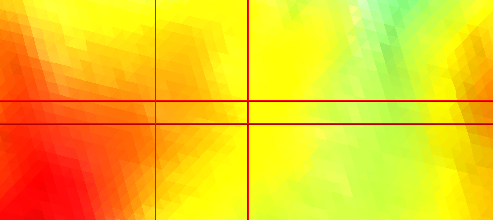
\includegraphics[width=13.7cm]{graphics/obr_ralek/hradek_vyrez.PNG}
\caption{Nahoře: pozice geometrie modelu (části úložiště) v rámci regionálního hydrogeologického modelu. Dole: detailní výřez; lze rozeznat jednotlivé elementy regionálního modelu (jejich velikost je cca 40 m).}
\label{hradek_piezo_head_orez}
\end{figure}

\newpage

\section{Výsledky, diskuze}
V další části textu je vždy uveden reprezentativní výběr obrázků k dané úloze. Víc obrázků je potom uvedeno v~Příloze. Kromě rozložení koncentrace v masivu sledujeme také průběh maximální koncentrace na vnější hranici (úložiště).

Varianty testovacích úloh slouží především pro otestování výpočetních možností a základní ověření správnosti fyzikálního modelu. Vstupní parametry, především materiálové vlastnosti hornin či zdrojové členy kontaminace, si v současné fázi nekladou za cíl být plně relistickými (snad kromě Varianty 3).

\subsection{Hydraulická úloha}
Všechny varianty testovacích úloh mají shodné rozložení hydraulického pole na oblasti. Hodnoty na hranici jsou rovny hodnotám z regionálního modelu (viz dolní detail na obr. \ref{hradek_piezo_head_orez}). Na obr. \ref{piezohead} je v horizontálním řezu oblastí (se zobrazenými puklinami) znázorněno rozložení piezometrické výšky spolu s rychlostním polem. Dle předpokladů dochází k většinovému proudění v edz kolem vrtů, a zřetelný je též drenážní vliv puklin.
\begin{figure}[H]
\centering
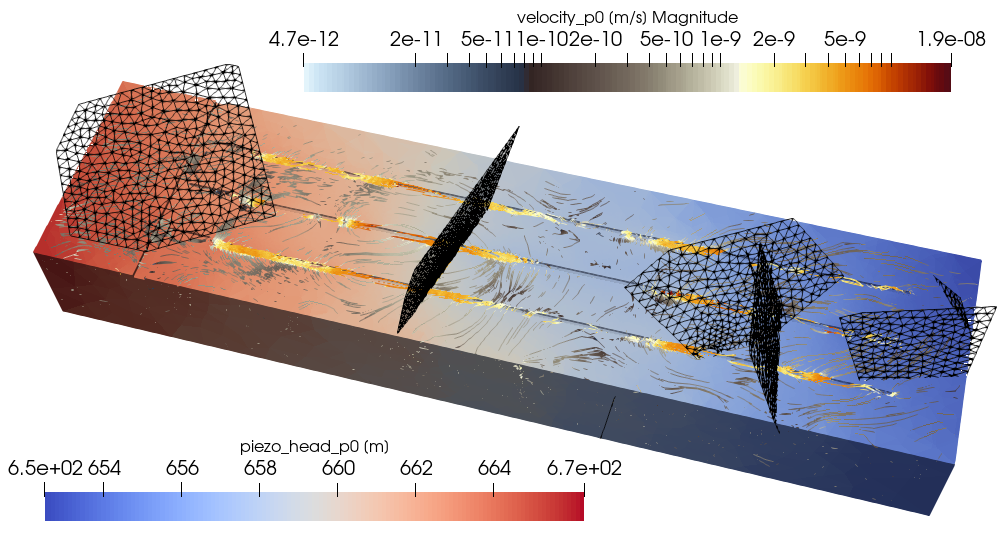
\includegraphics[width=16cm]{graphics/obr_ralek/hydro_s_pukl.png}
\caption{Rozložení piezometrické výšky a pole rychlostí na modelované oblasti. Horizontální řez s puklinami. Je zřetelný vliv puklin na rychlost a rozložení pole proudění.}
\label{piezohead}
\end{figure}

\newpage
\subsection{Varianta 1}
Na \obraz{var1}\footnote{Vyznění barevného zobrazení je do jisté míry ovlivněno numerickými oscilacemi. Podrobněji je problematika rozebrána u výsledků Varianty 2.} jsou v horizontálních řezech oblastí znázorněna rozložení pole koncentrací v~různých časech simulace. V souladu s předpokladem probíhá šíření kontaminantu přibližně "SV"~směrem, tj. ve směru převládajícího gradientu tlakové výšky, přičemž edz advekci zřetelně napomáhá.

\begin{figure}[H]
\centering

\includegraphics[clip,trim=0 {1cm} 0 0, width=16cm]{graphics/obr_ralek/nek_zdroj/01_3w.png}
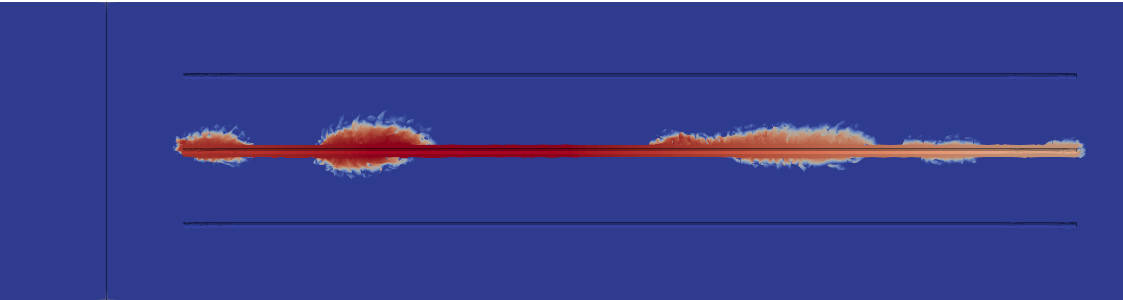
\includegraphics[clip,trim=0 {1cm} 0 0, width=16cm]{graphics/obr_ralek/nek_zdroj/04_3a.png}
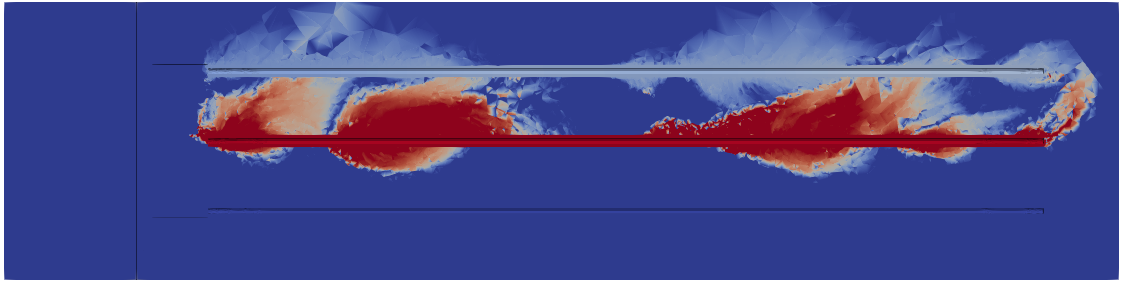
\includegraphics[clip,trim=0 {1cm} 0 0, width=16cm]{graphics/obr_ralek/nek_zdroj/06_20a.png}
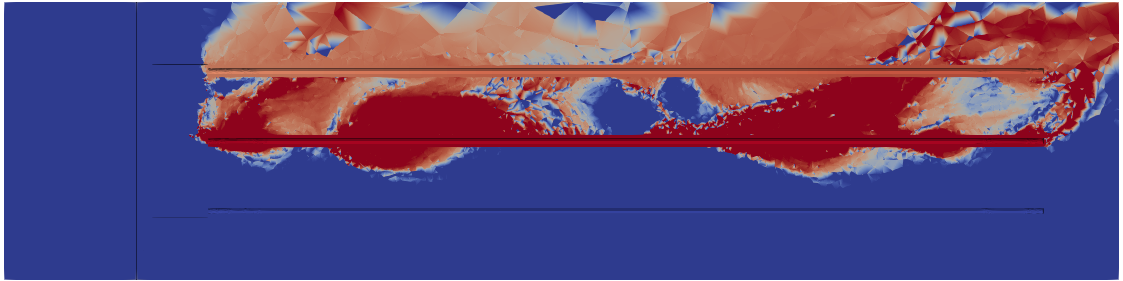
\includegraphics[clip,trim=0 {1cm} 0 0, width=16cm]{graphics/obr_ralek/nek_zdroj/08_300a.png}
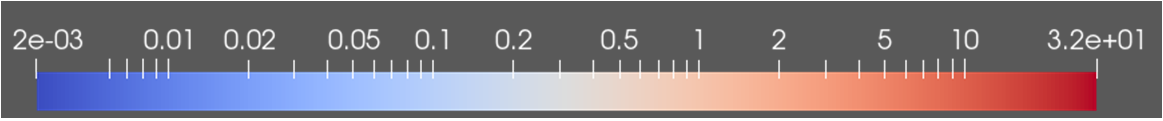
\includegraphics[width=16 cm]{graphics/obr_ralek/nek_zdroj/skala_nek_zdroj.png}
\caption{Prostorové rozložení koncentrace izotopu $^{129}I$ v~různých časech, odshora: 3 týdny, 3~roky, 20 let, 300 let; [$kg.m^{-3}$]. Varianta 1 ,horizontální řez oblastí.}
\label{var1}
\end{figure}

\subsection{Varianta 2}

Přes rozdíly ve zdrojovém členu kontaminace oproti variantě 1 (tok kontaminace na povrchu všech vrtů) probíhá šíření kontaminace \obraz{var2} podobně jako u varianty 1. Stejně tak vymývání kontaminace po vypnutí zdroje probíhá podobně "SV" směrem, se zřetelným vlivem puklin (jakési "tišiny" za puklinami), viz dolní dva řezy na obr. \ref{var2}.

\begin{figure}[H]
\centering
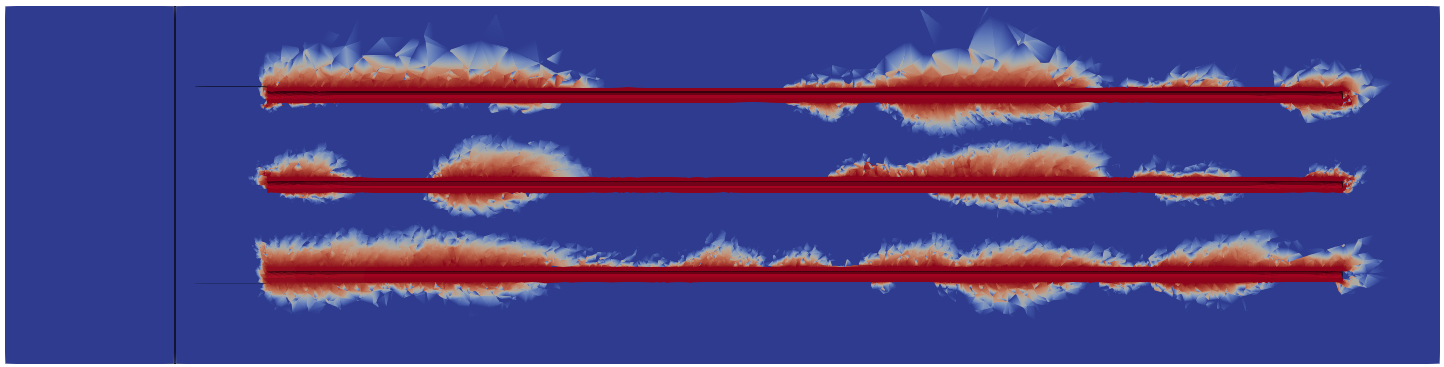
\includegraphics[width=16cm]{graphics/obr_ralek/var2/001a.png}
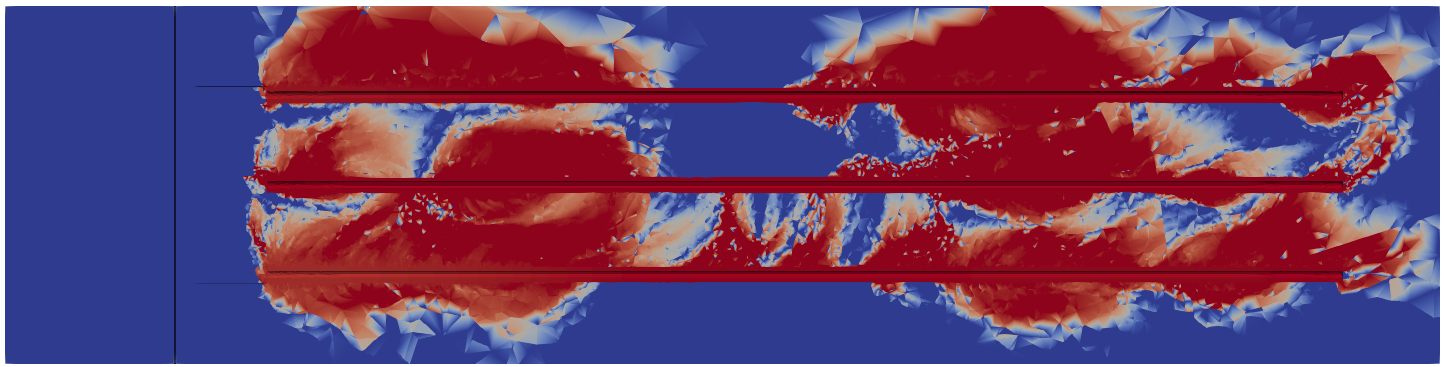
\includegraphics[width=16cm]{graphics/obr_ralek/var2/020a.png}
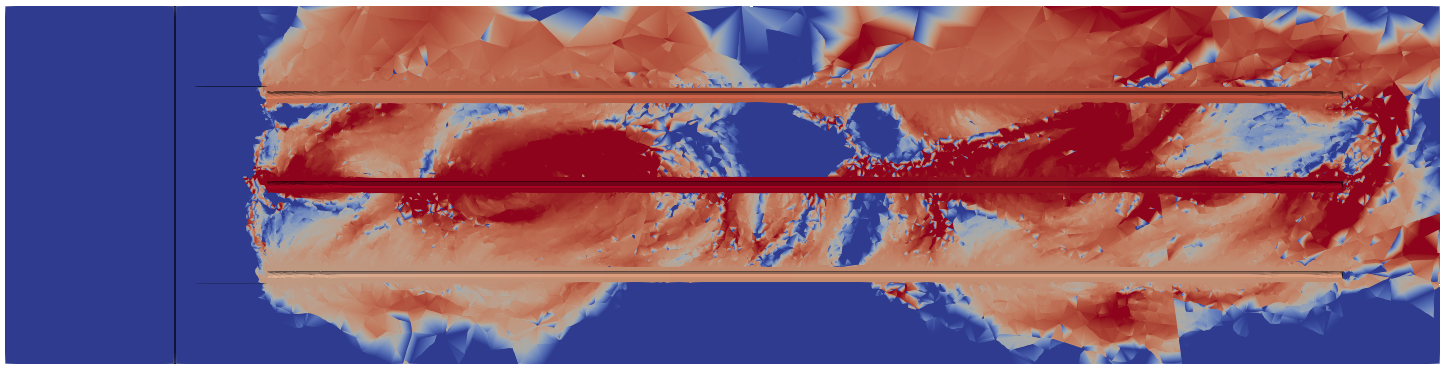
\includegraphics[width=16cm]{graphics/obr_ralek/var2/050a.png}
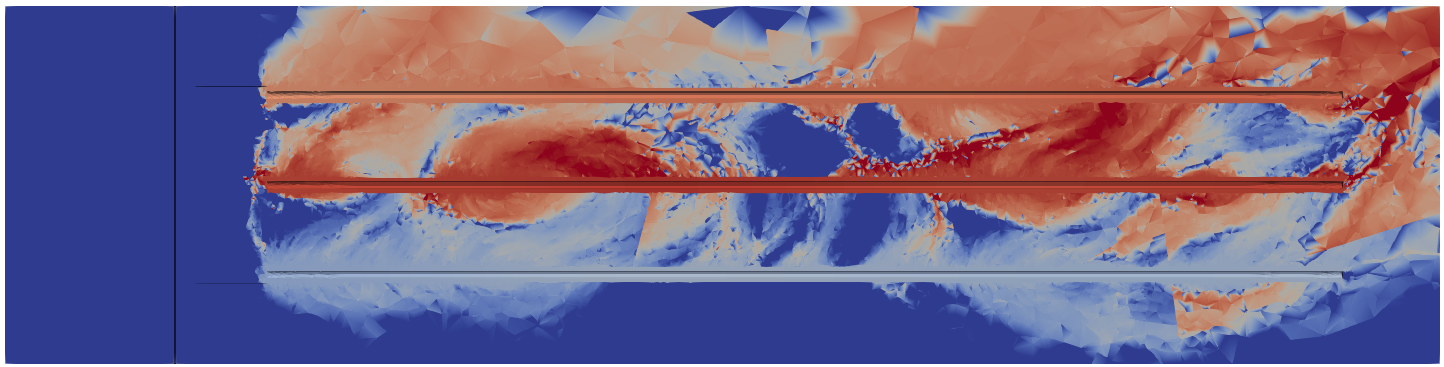
\includegraphics[width=16cm]{graphics/obr_ralek/var2/160a.png}
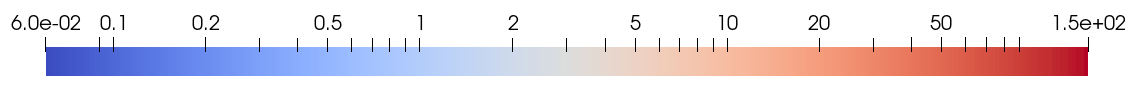
\includegraphics[width=16cm]{graphics/obr_ralek/var2/skala_var2.png}
\caption{Prostorové rozložení koncentrace izotopu $^{129}I$ v~různých časech, odshora: 1, 20, 50, 160 let; [$kg.m^{-3}$]. Varianta 2, horizontální řez oblastí.}
\label{var2}
\end{figure}

\newpage
\subsubsection{Numerické oscilace}
Jak již bylo zmíněno u varianty 1, na hodnoty koncentrace - a potažmo na vizualizace \obraz{threshold0-500} - má vliv numerických oscilací, kdy především na čele vlny šíření kontaminace se nacházejí nerealisticky vysoké hodnoty koncentrace (a naopak dále v masivu dochází k výskytu záporných koncentrací). Zřetelné je to při "rozjezdu" simulace (obr. \ref{oscilace_slice} nahoře), ovšem relikty těchto oscilací zůstávají i delší dobu (obr. \ref{oscilace_slice} dole  či obr. \ref{oscilace_3D} v Příloze), a především pak mohou ovlivnit vyhodnocení maximálních či průměrných koncentrací na hranici oblasti (viz sytě zelený element u horní hranice na obr. \ref{oscilace_slice} dole).

\begin{figure}[H]
\centering
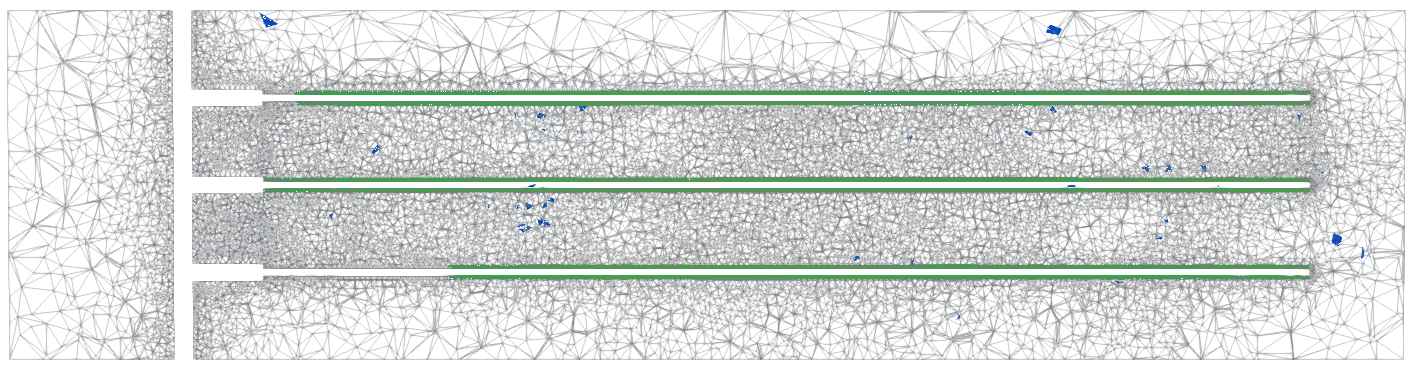
\includegraphics[width=16cm]{graphics/obr_ralek/var2/oscilace/slice01a.png}
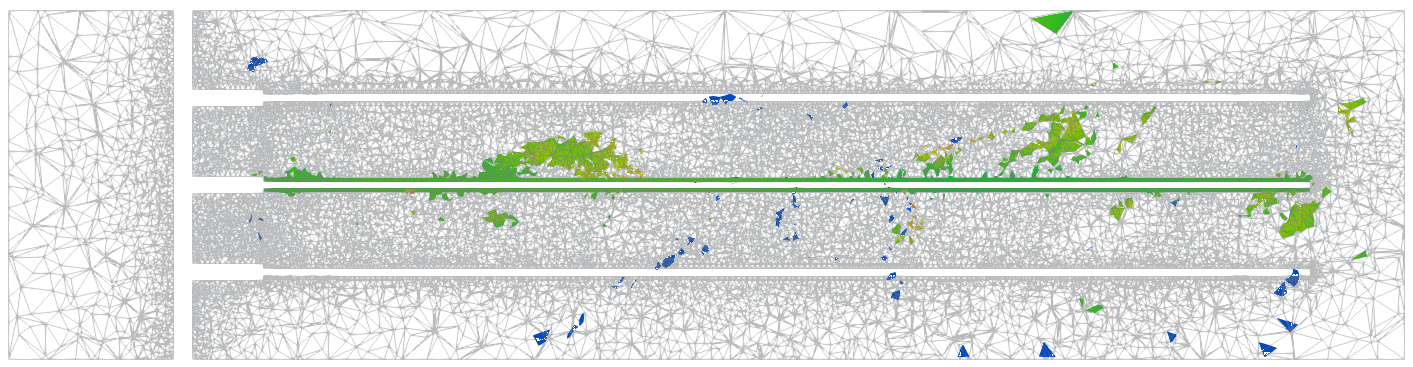
\includegraphics[width=16cm]{graphics/obr_ralek/var2/oscilace/slice40a.png}
\caption{Vliv numerických oscilací na postprocessing. Odstíny zelené odpovídají hodnotám koncentrace větším než ve zdroji, odstíny modré odpovídají záporným koncentracím. Nahoře: čas 1 rok, dole: 40 let. Varianta 2.}
\label{oscilace_slice}
\end{figure}

\begin{figure}[H]
\centering
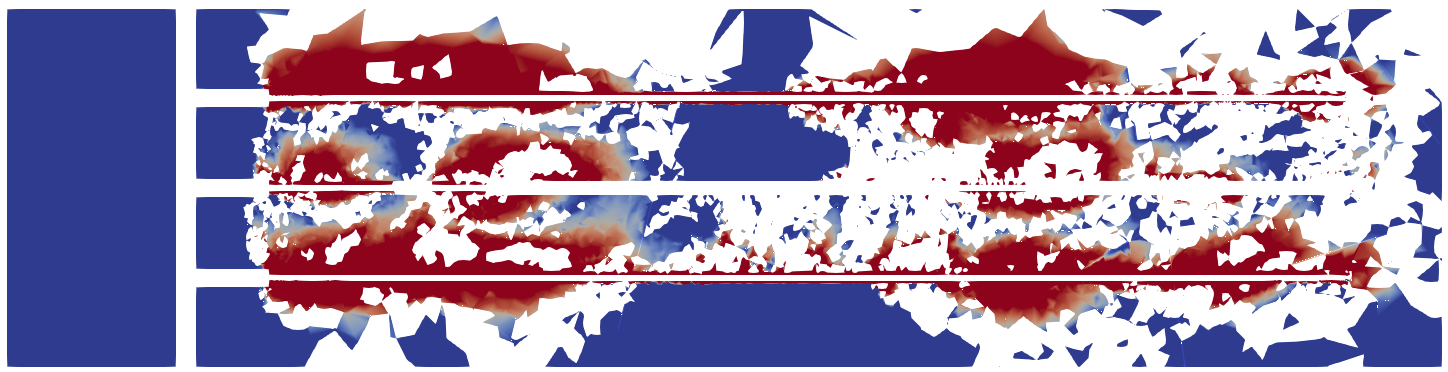
\includegraphics[width=16cm]{graphics/obr_ralek/var2/threshold0-500.png}
\caption{Rozložení koncentrace v čase 10 let s hodnotami bez záporných a 10\% nejvyšších hodnot.}
\label{threshold0-500}
\end{figure}

\newpage
\subsubsection{Hodnoty koncentrace na hranici oblasti} Časový průběh (maximální či průměrné) koncentrace na vnější hranici úložiště je jedním z~klíčo\-vých parametrů pro bezpečnostní analýzu úložiště. Jak bylo uvedeno výše, správné vyhodnocení může být negativně ovlivněno numerickými oscilacemi. Ty mohou v některých uzlech nabývat až o~několik (i desítek) řádů vyšších absolutních hodnot.

Pro připomenutí uvádíme, že zdrojový člen byl konstantní mezi 0-10 lety, poté byl nulový. V~grafu na obr. \ref{hranice_max_var2} jsou vyneseny časové průběhy maximální koncentrace na hranici oblasti a~její střední hodnoty pro všechna spočtená data. Kromě nereálně vysokých hodnot koncentrací či záporných středních hodnot pro prvních 10 let simulace je výrazný především kopcovitý charakter křivky maximálních hodnot, který (vzhledem k časovému rozsahu i rozdílem hodnot) nelze vyvětlit tak, že by na hranici přicházely vlny kontaminace po různých preferenčních cestách.

Odstraníme-li z množiny hodnot koncentrací na hranici horních a dolních např. 10\% hodnot (tj. vezmeme jen hodnoty ležící mezi kvantily 0.1 a 0.9), dostaneme křivku s mnohem lepší vypovídací hodnotou \obraz{hranice_max_var2_orez}. Maximální odezva na hranici nastává po cca 120 letech od začátku simulace, a to jak podle křivky maximálních hodnot, tak podle středních hodnot koncentrace. Chování křivky maximálních hodnot na obr. \ref{hranice_max_var2_orez} mezi lety 110-130 již lze odůvodnit postupným spojováním vln kontaminace z jednotlivých vrtů v "SV" rohu řezu oblastí. Této hypotéze by odpovídalo i zpomalení růstu střední hodnoty.

\begin{figure}[H]
\centering
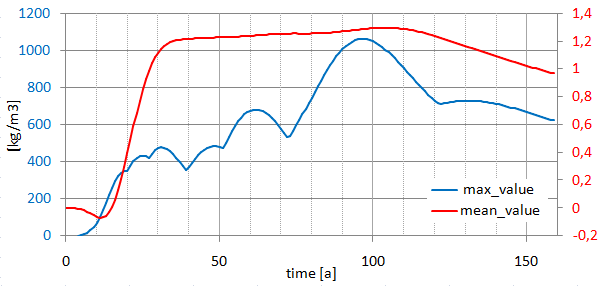
\includegraphics{graphics/obr_ralek/var2/hranice_max_var2.png}
\caption{Varianta 2 - časový průběh koncentrace na hranici oblasti (modře: maximální hodnoty, červeně: střední hodnoty).}
\label{hranice_max_var2}
\end{figure}

\begin{figure}[H]
\centering
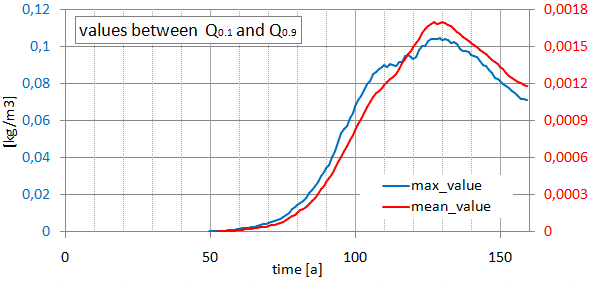
\includegraphics{graphics/obr_ralek/var2/hranice_max_orez.PNG}
\caption{Varianta 2 - časový průběh koncentrace na hranici oblasti (modře: maximální hodnoty, červeně: střední hodnoty). Z množiny dat v každém kroku odstraněno dolních a horních 10\% hodnot.}
\label{hranice_max_var2_orez}
\end{figure}

\subsection{Varianta 3}
Charakter zdroje kontaminace v této variantě již odpovídá reálné situaci postupného uvolňování radionuklidu $^{129}I$ z kontejneru a jeho prostupu bentonitovou vrstvou. Po prvotním nárůstu v~řádu několika desítek let dochází poté k postupnému poklesu v řádech tisíců let.

Vybrané časy simulace jsou znázorněny na obr. \ref{var3}. Charakter šíření kontaminace odpovídá variantě 2, pouze fáze vymývání je mnohem pozvolnější. Výsledky delší simulace než 1000 let nejsou prezentovány, neboť při prodloužení časového kroku numerické oscilace naprosto znehodnotily výsledky, což je zřejmé i z grafu maximálních nefiltrovaných hodnot koncentrace na hranici oblasti \obraz{hranice_max_var3}. Naproti tomu po ořezání dat o 10\% nejnižších a nejvyšších hodnot již časový vývoj maximální a průměrné koncentrace odpovídá očekávání, s maximální odezvou po cca 180 letech od maxima zdrojového členu.

\begin{figure}[H]
\centering
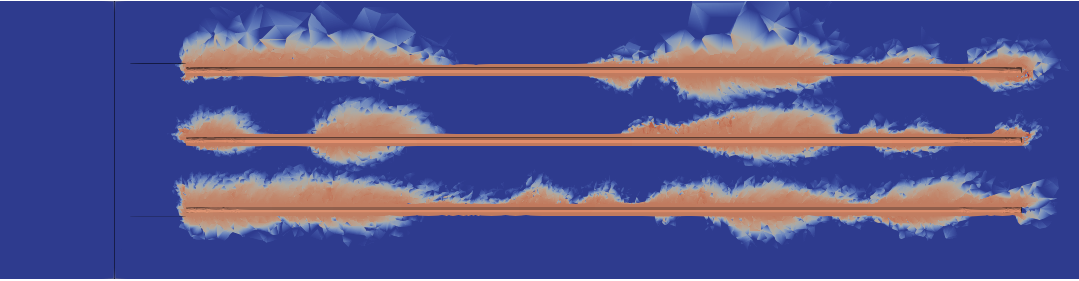
\includegraphics[width=16cm]{graphics/obr_ralek/var3/04_6y.png}
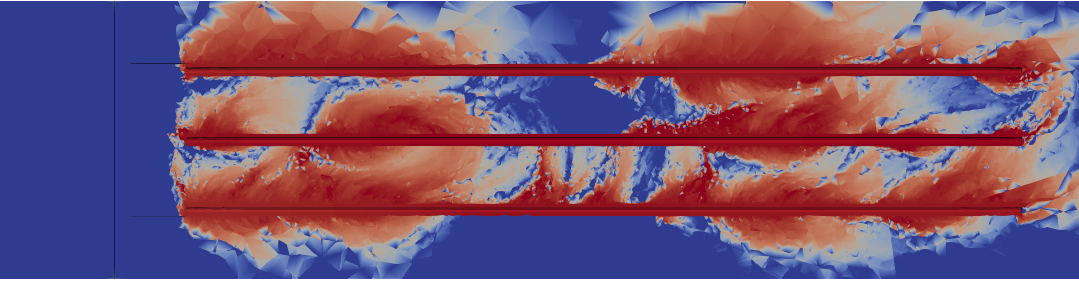
\includegraphics[width=16cm]{graphics/obr_ralek/var3/06_19y.png}
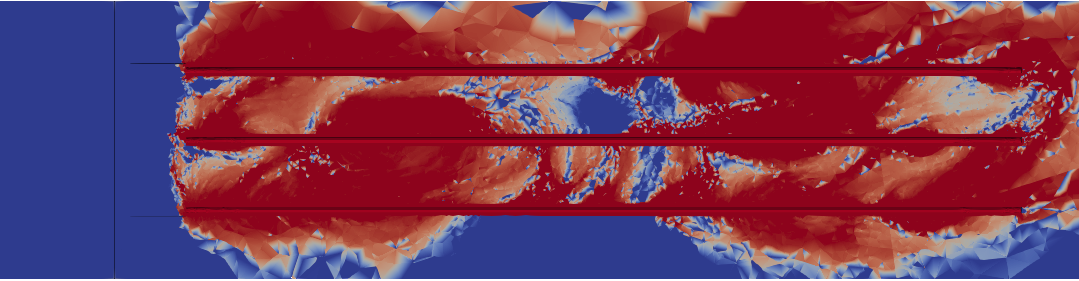
\includegraphics[width=16cm]{graphics/obr_ralek/var3/07_95y.png}
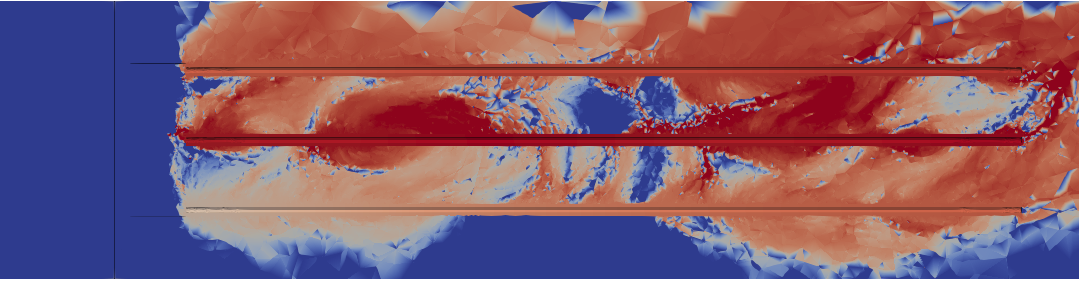
\includegraphics[width=16cm]{graphics/obr_ralek/var3/13_1046y.png}
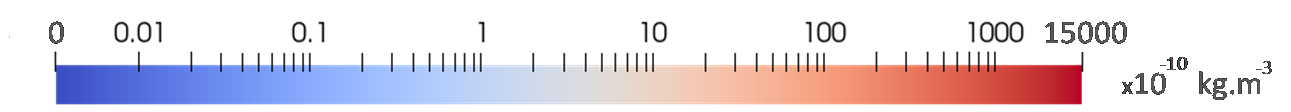
\includegraphics[width=16cm]{graphics/obr_ralek/var3/skala_nek_zdroj_vypnuti.png}   
\caption{Prostorové rozložení koncentrace izotopu $^{129}I$ v~různých časech, odshora: 6 let, 19 let, 95 let, 1046 let; [$kg.m^{-3}$]. Varianta 3, horizontální řez oblastí.}
\label{var3}
\end{figure}

\begin{figure}[H]
\centering
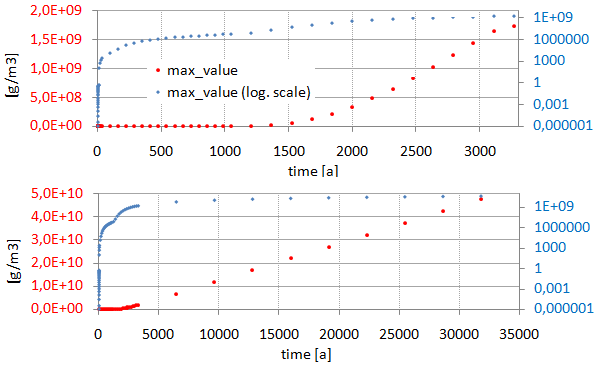
\includegraphics{graphics/obr_ralek/var3/hranice_max_var3.png}
\caption{Varianta 3 - časový průběh koncentrace na hranici oblasti (modře: maximální hodnoty, červeně: střední hodnoty).}
\label{hranice_max_var3}
\end{figure}

\begin{figure}[H]
\centering
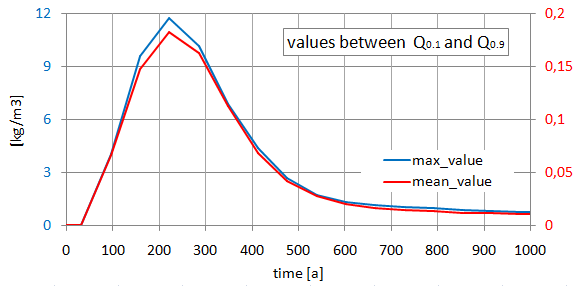
\includegraphics{graphics/obr_ralek/var3/var3_hranice_max_orez.PNG}
\caption{Varianta 3 - časový průběh koncentrace na hranici oblasti (modře: maximální hodnoty, červeně: střední hodnoty). Z množiny dat v každém kroku odstraněno dolních a horních 10\% hodnot.}
\label{hranice_max_orez}
\end{figure}

\newpage
\subsection{Současná verze modelu - nedostatky a možná řešení}
\label{detskenemoci}
Jak již bylo uvedeno v předchozím textu, současná verze modelu transportu se potýká s několika problémy, jejichž řešení však zároveň poskytuje prostor pro další rozvoj modelu. První dva mají společný jmenovatel ve využití knihoven síťovacího algoritmu GMSH \cite{gmsh} v našem kódu.
\begin{itemize}
 \item {\bf Reprezentace EDZ.} Je třeba nalézt způsob lepší reprezentace EDZ buďto specficky zjemněnou sítí, přepočtem efektivní vodivosti, nebo rozdělením modelu na dvě samostatné škály.
 \item {\bf Stabilita síťování.} Soušasné řízení kroku sítě vynucuje velká krok na celých puklinách což způsobuje neúspěch síťovače
 pro složitější průniky. Je třeba najít vhodný způsob precizního určování velikosti kroku sítě na různých částech geometrie.
 \item {\bf Numerické oscilace} zatěžují určení maximální koncentrace na hranici značnou chybou. Bude třeba optimalizovat parametry numerického schématu s ohledem na omezení oscilací při současném zachvání nízké numerické difúze.
 \item {\bf Nastavení OKP.} Použitá verze Flow123d neumožňuje současně volit prostorově proměnnou okrajouvou podmínku v kombinaci s časovou řadou zadanou ze souboru. Bude použita novější verze, která toto umožňuje.
\end{itemize}




\bibliographystyle{plain}
%\bibliographystyle{dinat-etal}
\bibliography{zprava.bib}

\section{Obrazová příloha}
\subsection{Varianta 1}
\begin{figure}[H]
\centering

\includegraphics[width=16cm]{graphics/obr_ralek/nek_zdroj/01_3w.png}
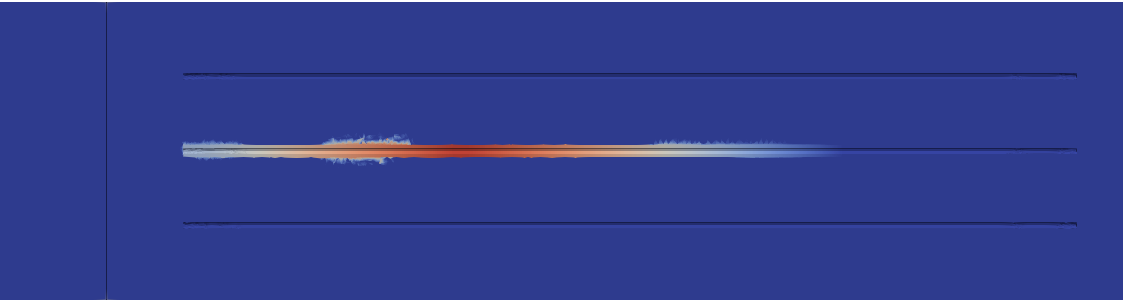
\includegraphics[width=16cm]{graphics/obr_ralek/nek_zdroj/02_4m.png}
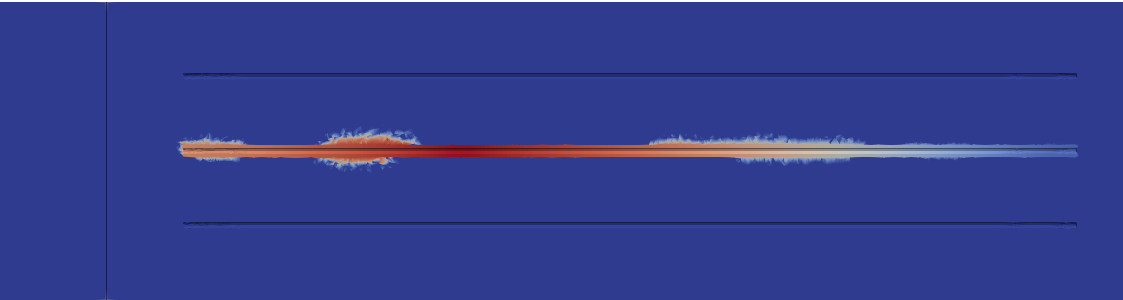
\includegraphics[width=16cm]{graphics/obr_ralek/nek_zdroj/03_1a.png}
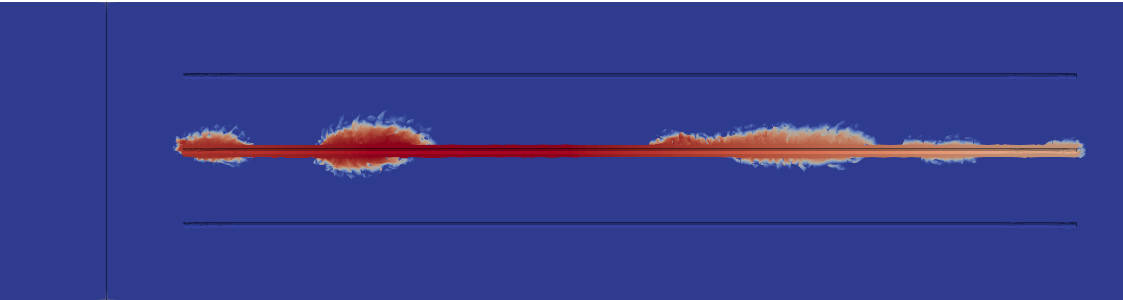
\includegraphics[width=16cm]{graphics/obr_ralek/nek_zdroj/04_3a.png}
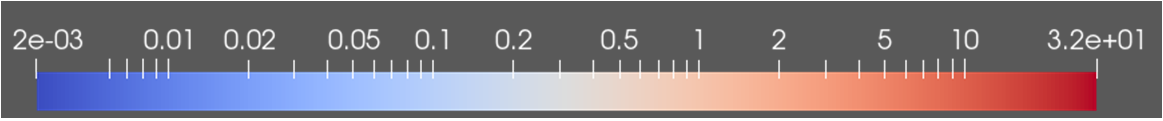
\includegraphics[width=16cm]{graphics/obr_ralek/nek_zdroj/skala_nek_zdroj.png}
\caption{Prostorové rozložení koncentrace izotopu $^{129}I$ v~různých časech, odshora: 3 týdny, 4 měsíce, 1 rok, 3 roky; [$kg.m^{-3}$]. Varianta 1, horizontální řez oblastí.}
\label{nek_zdroj_01}
\end{figure}

\begin{figure}[H]
\centering
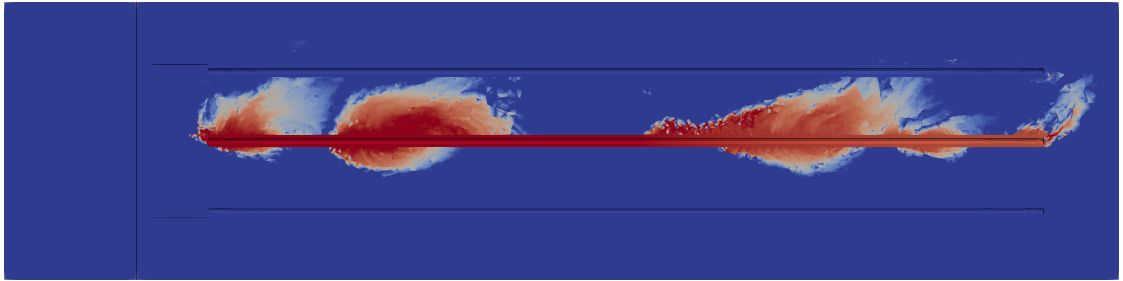
\includegraphics[width=16cm]{graphics/obr_ralek/nek_zdroj/05_6a.png}
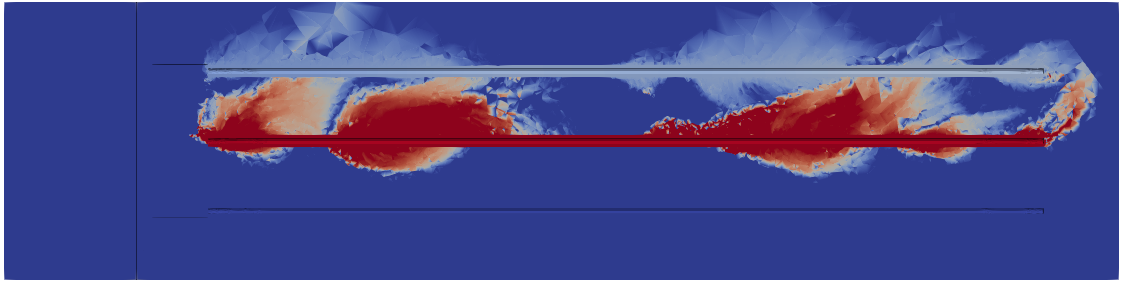
\includegraphics[width=16cm]{graphics/obr_ralek/nek_zdroj/06_20a.png}
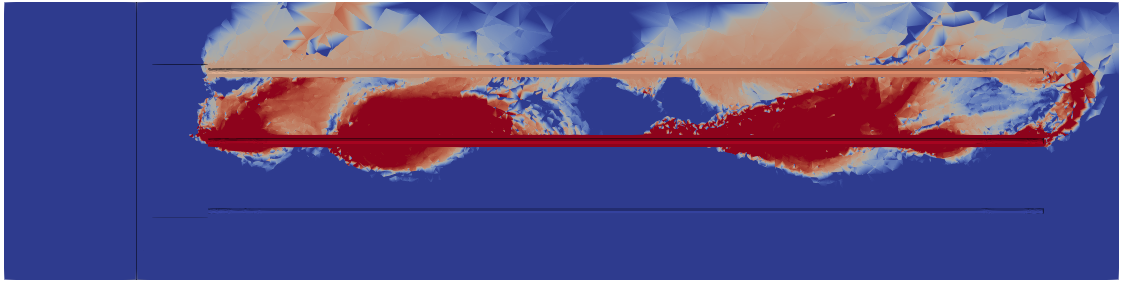
\includegraphics[width=16cm]{graphics/obr_ralek/nek_zdroj/07_50a.png}
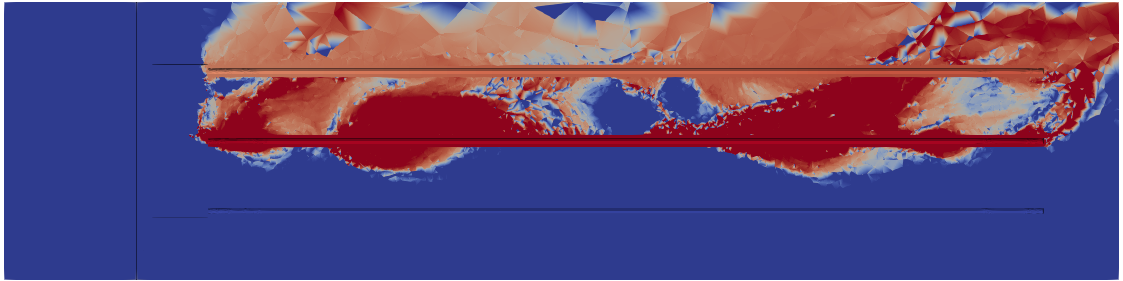
\includegraphics[width=16cm]{graphics/obr_ralek/nek_zdroj/08_300a.png}
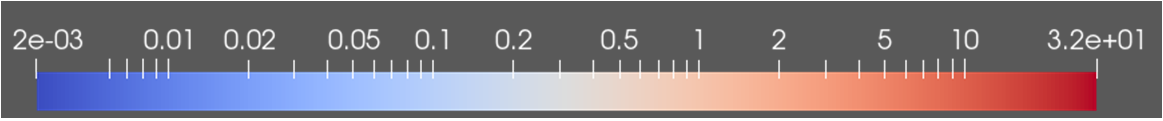
\includegraphics[width=16cm]{graphics/obr_ralek/nek_zdroj/skala_nek_zdroj.png}
\caption{Prostorové rozložení koncentrace izotopu $^{129}I$ v~různých časech, odshora: 6 let, 20 let, 50 let, 300 let; [$kg.m^{-3}$]. Varianta 1, horizontální řez oblastí.}
\label{nek_zdroj_02}
\end{figure}

\subsection{Varianta 2}
\begin{figure}[H]
\centering
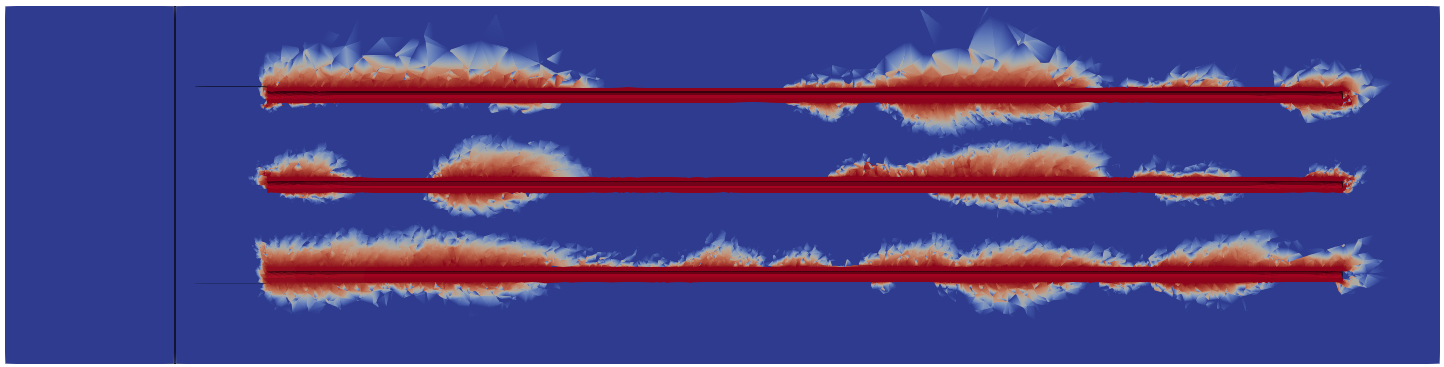
\includegraphics[width=16cm]{graphics/obr_ralek/var2/001a.png}
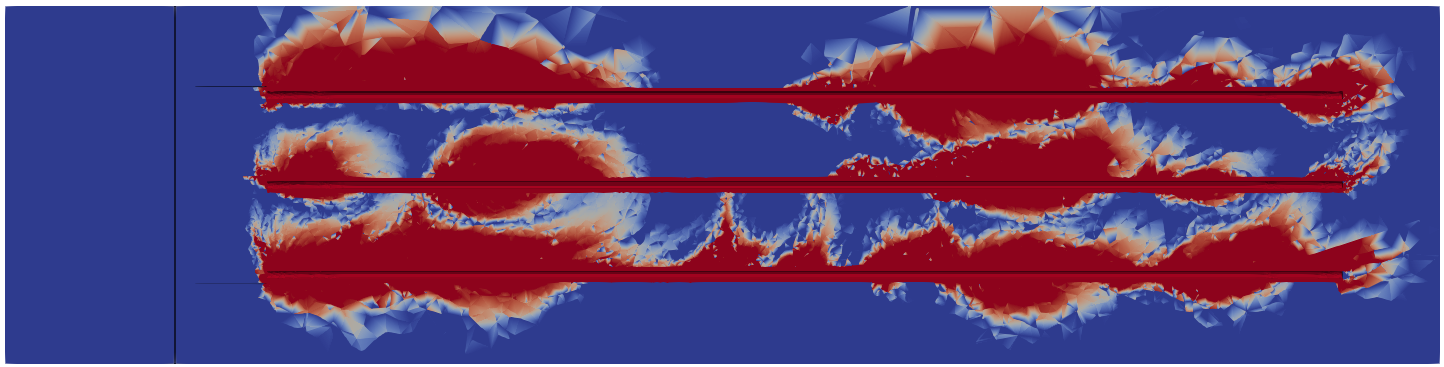
\includegraphics[width=16cm]{graphics/obr_ralek/var2/010a.png}
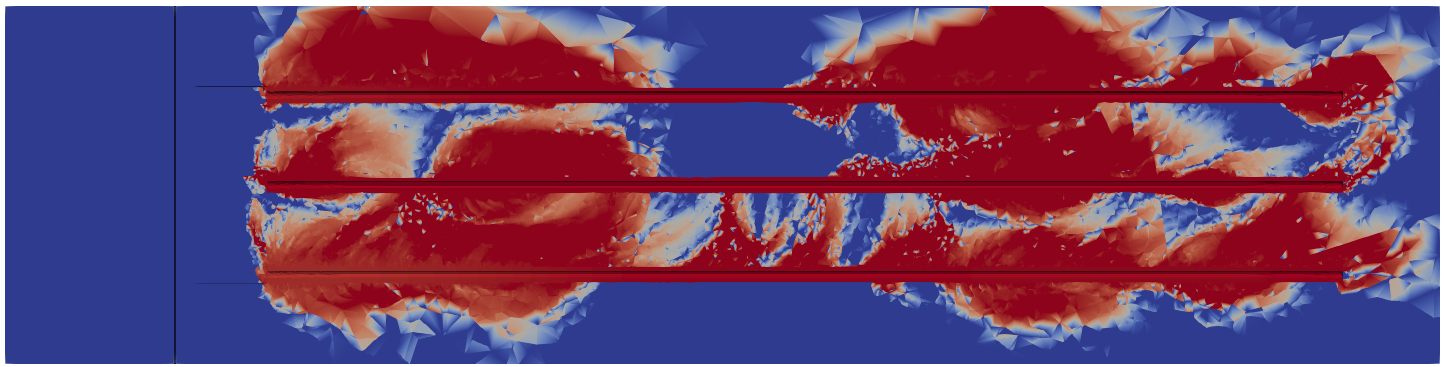
\includegraphics[width=16cm]{graphics/obr_ralek/var2/020a.png}
\includegraphics[width=16cm]{graphics/obr_ralek/var2/030a.png}
\includegraphics[width=16cm]{graphics/obr_ralek/var2/skala_var2.png}
\caption{Prostorové rozložení koncentrace izotopu $^{129}I$ v~různých časech, odshora: 1, 10, 20, 30 let; [$kg.m^{-3}$]. Varianta 2, horizontální řez oblastí.}
%\label{...}
\end{figure}

\begin{figure}[H]
\centering
\includegraphics[width=16cm]{graphics/obr_ralek/var2/050a.png}
\includegraphics[width=16cm]{graphics/obr_ralek/var2/070.png}
\includegraphics[width=16cm]{graphics/obr_ralek/var2/100a.png}
\includegraphics[width=16cm]{graphics/obr_ralek/var2/160a.png}
\includegraphics[width=16cm]{graphics/obr_ralek/var2/skala_var2.png}
\caption{Prostorové rozložení koncentrace izotopu $^{129}I$ v~různých časech, odshora: 50, 70, 100, 160 let; [$kg.m^{-3}$]. Varianta 2, horizontální řez oblastí.}
%\label{...}
\end{figure}

\begin{figure}[H]
\centering
\includegraphics[width=12cm]{graphics/obr_ralek/var2/oscilace/01a.png}
\includegraphics[width=12cm]{graphics/obr_ralek/var2/oscilace/10a.png}
\includegraphics[width=12cm]{graphics/obr_ralek/var2/oscilace/50a.png}
\includegraphics[width=12cm]{graphics/obr_ralek/var2/oscilace/150a.png}
\caption{Vliv numerických oscilací na postprocessing. Odstíny zelené odpovídají hodnotám koncentrace větším než ve zdroji, odstíny modré odpovídají záporným koncentracím. Odshora v časech: 1, 10, 50, 150 let. Varianta 2.}
\label{oscilace_3D}
\end{figure}

\begin{figure}[H]
\centering
\includegraphics[width=16cm]{graphics/obr_ralek/var2/oscilace/slice01a.png}
\includegraphics[width=16cm]{graphics/obr_ralek/var2/oscilace/slice10a.png}
\includegraphics[width=16cm]{graphics/obr_ralek/var2/oscilace/slice40a.png}
\includegraphics[width=16cm]{graphics/obr_ralek/var2/oscilace/slice150a.png}
\caption{Vliv numerických oscilací na postprocessing. Odstíny zelené odpovídají hodnotám koncentrace větším než ve zdroji, odstíny modré odpovídají záporným koncentracím. Odshora v časech: 1, 10, 40, 150 let. Varianta 2.}
%\label{oscilace_slice}
\end{figure}

\subsection{Varianta 3}
\begin{figure}[H]
\centering
\includegraphics[width=16cm]{graphics/obr_ralek/var3/02_1y.png}
\includegraphics[width=16cm]{graphics/obr_ralek/var3/04_6y.png}
\includegraphics[width=16cm]{graphics/obr_ralek/var3/06_19y.png}
\includegraphics[width=16cm]{graphics/obr_ralek/var3/07_95y.png}
\includegraphics[width=16cm]{graphics/obr_ralek/var3/skala_nek_zdroj_vypnuti.png}
\caption{Prostorové rozložení koncentrace izotopu $^{129}I$ v~různých časech, odshora: 1 rok, 6 let, 19 let, 95 let; [$kg.m^{-3}$]. Varianta 3, horizontální řez oblastí.}
\label{nek_zdroj_vyp_01}
\end{figure}

\begin{figure}[H]
\centering
\includegraphics[width=16cm]{graphics/obr_ralek/var3/08_158y.png}
\includegraphics[width=16cm]{graphics/obr_ralek/var3/09_222y.png}
\includegraphics[width=16cm]{graphics/obr_ralek/var3/10_285y.png}
\includegraphics[width=16cm]{graphics/obr_ralek/var3/13_1046y.png}
\includegraphics[width=16cm]{graphics/obr_ralek/var3/skala_nek_zdroj_vypnuti.png}
\caption{Prostorové rozložení koncentrace izotopu $^{129}I$ v~různých časech, odshora: 158 let, 222 let, 285 let, 1046 let; [$kg.m^{-3}$]. Varianta 3, horizontální řez oblastí.}
\label{nek_zdroj_vyp_02}
\end{figure}

\end{onehalfspacing} 

\end{document}
